% !TeX root = booklet-03.tex
\BookletReview{notes/booklet-03/prerequisites}
\ifCompleteNotes\else
\setcounter{chapter}{1}
\chapter{مشخصه انتقال ولتاژ در مدارهای منطقی}
\fi
\setcounter{section}{4}
\section{مشخصه انتقال \lr{DC}}
\label{sec:dc-transfer}
در \lr{DC Transfer Characteristic}، برای هر ولتاژ ورودی، خروجی
مدار را پس از رسیدن به حالت ماندگار تعیین می‌کنیم. فرض می‌شود
ورودی آن‌قدر آهسته تغییر می‌کند که ظرفیت‌ها فرصت شارژ و تخلیه
داشته باشند. مدار دیجیتال نیز از ولتاژها و جریان‌های پیوسته
ساخته شده است. تفسیر منطقی، بازه‌هایی از این ولتاژها را به صفر
و یک نسبت می‌دهد \cite[مقدمه بخش \secnum{۲.۵}، صفحه ۸۷]{weste}.
% !TeX root = booklet-03.tex
\subsection{مشخصه \lr{DC} یک \lr{Static CMOS Inverter}}
\label{sec:inverter-dc}
هدف این بخش، محاسبه \(V_{\mathrm{out}}\) برای هر
\(V_{\mathrm{in}}\) است. مبنای مدار و تقسیم‌بندی، بخش
\secnum{۲.۵.۱} کتاب و اسلایدهای ۳ تا ۷ است
\cite{weste,dcslides}. ابتدا قراردادهای عمومی ولتاژ و جریان را
می‌نویسیم. استخراج پنج ناحیه با مدل متقارن کتاب انجام می‌شود.

\subsubsection{مدار، فرض‌ها و قرارداد علامت}
\label{sec:inverter-conventions}
در شکل \ref{fig:inverter-circuit}، سورس \lr{nMOS} به زمین و سورس
\lr{pMOS} به \(V_{DD}\) متصل است. گیت‌ها به یک ورودی و درین‌ها
به یک خروجی وصل‌اند. بدنه \lr{nMOS} را به زمین و بدنه
\lr{pMOS} را به تغذیه می‌بندیم. پس اختلاف ولتاژ سورس و بدنه برای
هر دو صفر است و تغییر آستانه ناشی از بایاس بدنه در این مدار ایجاد
نمی‌شود. فرض می‌کنیم \(0\le V_{\mathrm{in}},V_{\mathrm{out}}\le V_{DD}\).
\begin{figure}[!htbp]
\centering
\begin{latin}
\PersianMathDigits
\begin{circuitikz}[scale=1,transform shape]
\draw (3,1.3) node[nmos] (n) {};
\draw (3,3.7) node[pmos] (p) {};
\draw (n.S)--(3,0.3) node[ground] {};
\draw (p.S)--(3,4.7) node[ocirc] {} node[above] {\(V_{DD}\)};
\draw (n.D)--(p.D);
\draw (n.G)--(1.3,1.3)--(1.3,3.7)--(p.G);
\draw (1.3,2.5) node[circ] {}--(0.4,2.5) node[ocirc] {}
 node[left] {\(V_{\mathrm{in}}\)};
\draw (3,2.5) node[circ] {}--(5,2.5) node[ocirc] {}
 node[right] {\(V_{\mathrm{out}}\)};
\draw[->] (4.8,4.2)--(4.8,3.3) node[midway,right] {\(I_p\)};
\draw[->] (4.8,1.8)--(4.8,0.9) node[midway,right] {\(I_n\)};
\node[right] at (3.3,3.7) {pMOS};
\node[right] at (3.3,1.3) {nMOS};
\end{circuitikz}
\end{latin}
\caption{بازترسیم آموزشی مدار شکل \secnum{۲.۲۵} کتاب و اسلاید ۳.
پیکان‌ها بزرگی جریان‌های بالاکش و پایین‌کش را نشان می‌دهند.
بدنه‌ها به سورس‌های متناظر متصل‌اند.}
\label{fig:inverter-circuit}
\end{figure}

با تعریف اختلاف ولتاژ پایانه‌ها، روابط \lr{nMOS} چنین‌اند
\begin{equation}
 V_{GS,n}=V_{\mathrm{in}},\qquad
 V_{DS,n}=V_{\mathrm{out}}.
 \label{eq:inverter-n-voltages}
\end{equation}
برای \lr{pMOS}، قرارداد علامت‌دار کتاب و قرارداد بزرگی مثبت به‌ترتیب
به صورت زیر به هم مربوط‌اند
\begin{align}
 V_{GS,p}&=V_{\mathrm{in}}-V_{DD},&
 V_{DS,p}&=V_{\mathrm{out}}-V_{DD},
 \label{eq:inverter-p-signed}\\
 V_{SG,p}&=V_{DD}-V_{\mathrm{in}}=-V_{GS,p},&
 V_{SD,p}&=V_{DD}-V_{\mathrm{out}}=-V_{DS,p}.
 \label{eq:inverter-p-magnitudes}
\end{align}
آستانه \lr{nMOS} را \(V_{tn}>0\) و آستانه علامت‌دار
\lr{pMOS} را \(V_{tp}<0\) می‌نامیم. بزرگی آستانه را به صورت زیر
تعریف می‌کنیم.
\[
 V_{TP}=|V_{tp}|=-V_{tp},\qquad V_{TP}>0.
\]
برای جریان نیز
\(I_n=I_{DS,n}\ge0\) و \(I_p=|I_{DS,p}|\ge0\) به کار می‌روند.
با جهت جریان درین به سورس، \(I_{DS,p}=-I_p\) است.

خروجی را بدون جریان بار \lr{DC} فرض می‌کنیم. در حالت ماندگار،
\lr{KCL} به رابطه اصلی تحلیل می‌انجامد
\begin{equation}
 \boxed{I_n(V_{\mathrm{in}},V_{\mathrm{out}})
       =I_p(V_{\mathrm{in}},V_{\mathrm{out}})}.
 \label{eq:inverter-kcl}
\end{equation}
جریان تغذیه در این مدل همان \(I_{DD}=I_p=I_n\) است. وجود ظرفیت
خروجی با این شرط ماندگار سازگار است. اگر بار جریان ثابت یا مقاومتی
داشته باشد، باید \(I_L\) را در معادله گره وارد کرد.

برای استخراج اصلی، فرض‌های متقارن کتاب را به کار می‌بریم
\begin{equation}
 V_{tn}=V_{TP}=V_t>0,\qquad
 \beta_n=\beta_p=\beta>0,\qquad V_{DD}>2V_t.
 \label{eq:inverter-symmetry}
\end{equation}
مدل، \lr{Long-channel Shockley} با آستانه و \lr{Mobility} ثابت است.
در استخراج ایده‌آل، \lr{CLM} و نشتی صفر فرض می‌شوند. شرط آخر،
بازه‌ای برای روشن‌بودن هم‌زمان دو افزاره ایجاد می‌کند. اگر تغذیه
از مجموع بزرگی دو آستانه کمتر باشد، ترتیب پنج‌ناحیه‌ای حاضر
نیازمند بازنگری است و جریان زیرآستانه نیز می‌تواند تعیین‌کننده شود.

پارامتر \(\beta\) با واحد \(\unit{\ampere\per\volt\squared}\)
از \(\beta=\mu C_{\mathrm{ox}}W/L\) به دست می‌آید. با
\(C_{\mathrm{ox}}\) و طول یکسان، برابری دو \(\beta\) نیازمند
\(\mu_nW_n=\mu_pW_p\) است. کتاب برای جبران \lr{Mobility}
کمتر حفره‌ها، عرض \lr{pMOS} حدود دو تا سه برابر \lr{nMOS} را در
تقریب این بخش مطرح می‌کند \cite[صفحه ۸۸]{weste}. این نسبت،
تقریب همان بحث است و مقدار دقیق به فناوری و بایاس وابسته است.

\subsubsection{مدل جریان و تبدیل شرط‌های ناحیه کاری}
\label{sec:inverter-regions}
برای خوانایی روابط، اضافه‌ولتاژهای مثبت را تعریف می‌کنیم
\begin{equation}
 a=V_{\mathrm{in}}-V_{tn},\qquad
 b=V_{DD}-V_{\mathrm{in}}-V_{TP},\qquad
 y=V_{\mathrm{out}},\qquad u=V_{DD}-y.
 \label{eq:inverter-ab-definitions}
\end{equation}
کمیت \(u\) افت ولتاژ سورس به درین \lr{pMOS} است. نمادهای
\(a,b\) با واحد ولت‌اند و تنها وقتی مثبت باشند افزاره متناظر
در مدل هدایت قوی روشن است. روابط جریان مدل مربعی کتاب با این
نمادها چنین نوشته می‌شوند
\begin{equation}
 I_n=
 \begin{cases}
 0,&a\le0,\\[2pt]
 \beta_n(ay-y^2/2),&a>0,\quad 0\le y<a,\\[2pt]
 \beta_n a^2/2,&a>0,\quad y\ge a,
 \end{cases}
 \label{eq:inverter-n-current}
\end{equation}
و برای بزرگی جریان \lr{pMOS} داریم
\begin{equation}
 I_p=
 \begin{cases}
 0,&b\le0,\\[2pt]
 \beta_p(bu-u^2/2),&b>0,\quad 0\le u<b,\\[2pt]
 \beta_p b^2/2,&b>0,\quad u\ge b.
 \end{cases}
 \label{eq:inverter-p-current}
\end{equation}
این روابط از مدل بخش \secnum{۲.۲} کتاب با قراردادهای جدول
\secnum{۲.۲} به دست آمده‌اند \cite[صفحات ۶۶ و ۸۸]{weste}.
در مرز \(y=a\) یا \(u=b\)، دو شاخه روشن، جریان یکسانی می‌دهند.
برای نمونه، \(\beta_n[a(a)-a^2/2]=\beta_na^2/2\).
نسبت‌دادن نقطه مرزی به شاخه اشباع، قرارداد این جزوه است.
در آستانه دقیق، جریان ایده‌آل صفر است.

برای \lr{nMOS} روشن، شرط اشباع
\(V_{DS,n}\ge V_{GS,n}-V_{tn}\) مستقیماً می‌دهد
\(y\ge V_{\mathrm{in}}-V_{tn}\).
برای \lr{pMOS} روشن، از بزرگی ولتاژها شروع می‌کنیم
\begin{align}
 V_{SD,p}&\ge V_{SG,p}-V_{TP},\notag\\
 V_{DD}-y&\ge V_{DD}-V_{\mathrm{in}}-V_{TP},\notag\\
 -y&\ge -V_{\mathrm{in}}-V_{TP},\notag\\
 \boxed{y\le V_{\mathrm{in}}+V_{TP}}.
 \label{eq:inverter-p-saturation-condition}
\end{align}
در مرحله آخر، ضرب در منفی یک، جهت نامساوی را عوض کرده است.
با \(V_{TP}=-V_{tp}\)، این شرط برابر
\(y\le V_{\mathrm{in}}-V_{tp}\) در قرارداد کتاب است.
جدول \ref{tab:inverter-device-regions} همه شرط‌ها را جمع می‌کند
\cite[جدول \secnum{۲.۲}]{weste}\cite[اسلایدهای ۵ و ۶]{dcslides}.
\begin{table}[!htbp]
\centering
\small
\caption{شرط‌های ناحیه کاری در مختصات ورودی و خروجی.
در ردیف‌های روشن، شرط روشن‌بودن نیز باید برقرار باشد.}
\label{tab:inverter-device-regions}
\begin{tabularx}{\linewidth}{cc>{\raggedleft\arraybackslash}X}
\toprule
افزاره & ناحیه & شرط\\
\midrule
\lr{nMOS} & \lr{Cutoff} & \(V_{\mathrm{in}}\le V_{tn}\)\\
\lr{nMOS} & \lr{Linear} & \(V_{\mathrm{in}}>V_{tn},\quad 0\le y<V_{\mathrm{in}}-V_{tn}\)\\
\lr{nMOS} & \lr{Saturation} & \(V_{\mathrm{in}}>V_{tn},\quad y\ge V_{\mathrm{in}}-V_{tn}\)\\
\lr{pMOS} & \lr{Cutoff} & \(V_{\mathrm{in}}\ge V_{DD}-V_{TP}\)\\
\lr{pMOS} & \lr{Linear} & \(V_{\mathrm{in}}<V_{DD}-V_{TP},\quad y>V_{\mathrm{in}}+V_{TP}\)\\
\lr{pMOS} & \lr{Saturation} & \(V_{\mathrm{in}}<V_{DD}-V_{TP},\quad y\le V_{\mathrm{in}}+V_{TP}\)\\
\bottomrule
\end{tabularx}
\end{table}

در یک ورودی مشخص، انتخاب ناحیه به خروجی مجهول هم وابسته است.
بنابراین، روش حل چنین است. یک ترکیب ناحیه را فرض می‌کنیم، جریان‌های
متناظر را برابر می‌گذاریم و خروجی را حساب می‌کنیم. سپس همه شرط‌های
آن ترکیب را با خروجی به‌دست‌آمده می‌سنجیم. اگر شرطی نقض شود،
شاخه دیگری باید بررسی شود.

\subsubsection{روش ترسیمی و تقاطع منحنی‌های جریان}
\label{sec:inverter-graphical}
در ورودی ثابت، \(a\) و \(b\) ثابت‌اند. اگر خروجی \(y\) را از
صفر تا تغذیه تغییر دهیم، جریان \lr{nMOS} ابتدا افزایش می‌یابد و
سپس در مدل ایده‌آل ثابت می‌شود. برای \lr{pMOS}، افزایش خروجی،
\(u=V_{DD}-y\) را کم می‌کند. جریان آن ابتدا می‌تواند در اشباع
ثابت باشد و سپس تا صفر کاهش یابد. نقطه تقاطع دو منحنی شرط
\eqref{eq:inverter-kcl} را برآورده می‌کند. با تکرار این کار برای
ورودی‌های مختلف، مشخصه انتقال به دست می‌آید
\cite[شکل \secnum{۲.۲۶}]{weste}.

شکل \ref{fig:inverter-current-intersection} نمونه آموزشی این ساخت
ترسیمی است. پارامترهای فرضی آن
\(V_{DD}=\qty{1.2}{\volt}\)، \(V_t=\qty{0.3}{\volt}\)،
\(\beta_n=\beta_p=\qty{200}{\micro\ampere\per\volt\squared}\)
و \(V_{\mathrm{in}}=\qty{0.5}{\volt}\) هستند.
پس \(a=\qty{0.2}{\volt}\) و \(b=\qty{0.4}{\volt}\) است.
حد جریان اشباع \lr{nMOS} برابر \(\qty{4}{\micro\ampere}\) و حد
متناظر \lr{pMOS} برابر \(\qty{16}{\micro\ampere}\) است.
تقاطع در \(y\approx\qty{1.1464}{\volt}\) و
\(I_n=I_p=\qty{4}{\micro\ampere}\) رخ می‌دهد.
\begin{figure}[!htbp]
\centering
\begin{latin}
\PersianMathDigits
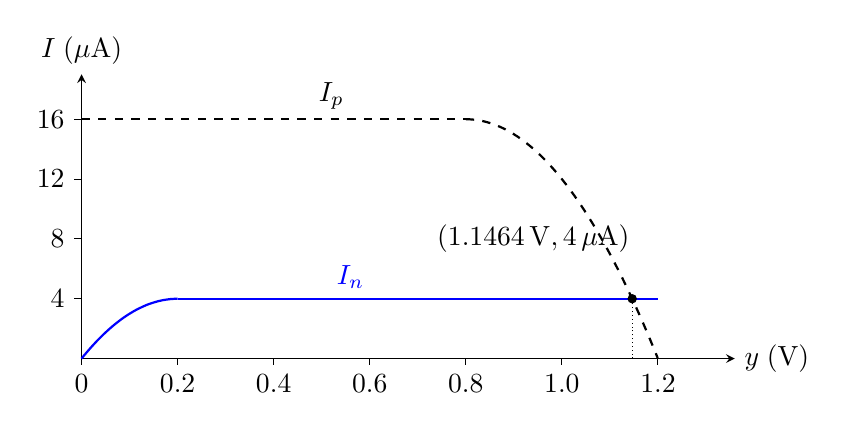
\begin{tikzpicture}[x=6.1cm,y=0.19cm,>=stealth]
\draw[->] (0,0)--(1.36,0) node[right] {\(y\;(\mathrm{V})\)};
\draw[->] (0,0)--(0,19) node[above] {\(I\;(\mu\mathrm{A})\)};
\foreach \x in {0,0.2,0.4,0.6,0.8,1.0,1.2}
 {\draw (\x,0)--(\x,-0.4) node[below] {\(\x\)};}
\foreach \y in {4,8,12,16}
 {\draw (0,\y)--(-0.015,\y) node[left] {\(\y\)};}
\draw[thick,blue,domain=0:0.2,samples=40]
 plot (\x,{200*(0.2*\x-\x*\x/2)});
\draw[thick,blue] (0.2,4)--(1.2,4);
\draw[thick,dashed] (0,16)--(0.8,16);
\draw[thick,dashed,domain=0.8:1.2,samples=45]
 plot (\x,{200*(0.4*(1.2-\x)-(1.2-\x)^2/2)});
\draw[densely dotted] (1.146410,0)--(1.146410,4);
\fill (1.146410,4) circle[radius=1.7pt];
\node[blue,above] at (0.56,4) {\(I_n\)};
\node[above] at (0.52,16) {\(I_p\)};
\node[anchor=west] at (0.72,8) {\((1.1464\,\mathrm{V},4\,\mu\mathrm{A})\)};
\end{tikzpicture}
\end{latin}
\caption{تقاطع جریان‌ها برای یک ورودی فرضی در مدل مربعی متقارن.
ساخت نمودار بر اساس روش شکل \secnum{۲.۲۶} کتاب است.}
\label{fig:inverter-current-intersection}
\end{figure}

جهت تغییر خروجی را نیز می‌توان از همین شکل فهمید. اگر در این
مثال \(y\) از مقدار تعادل کمتر شود، \(I_p>I_n\) و ظرفیت خروجی
شارژ می‌شود. اگر خروجی از تعادل بالاتر برود، \(I_n>I_p\) و خروجی
تخلیه می‌شود. این استدلال، بازگشت خروجی به تعادل را در همسایگی
نقطه نشان می‌دهد. در حالت استثنایی که دو منحنی در بازه‌ای کاملاً
روی هم قرار گیرند، مدل ایده‌آل خروجی یکتا نمی‌دهد. ناحیه \lr{C}
همین حالت را دارد.

\subsubsection{استخراج تحلیلی پنج ناحیه}
\label{sec:inverter-five-regions}
در ادامه فرض‌های \eqref{eq:inverter-symmetry} برقرارند، پس
\(a=V_{\mathrm{in}}-V_t\) و
\(b=V_{DD}-V_{\mathrm{in}}-V_t\) هستند. ترتیب نام‌های
\lr{A} تا \lr{E} از جدول \secnum{۲.۳} کتاب و اسلاید ۷ گرفته
شده است \cite{weste,dcslides}. نام ناحیه مدار، ترکیب ناحیه کاری
دو افزاره را مشخص می‌کند.

\paragraph*{ناحیه \lr{A} و خروجی بالا}
برای \(0\le V_{\mathrm{in}}\le V_t\)، ترانزیستور \lr{nMOS}
در مدل ایده‌آل جریان صفر دارد. چون \(V_{DD}>2V_t\)، ترانزیستور
\lr{pMOS} روشن است. شرط \lr{KCL}، جریان آن را نیز صفر می‌کند.
در شاخه \lr{Linear}، معادله جریان آن چنین است
\[
 0=\beta(bu-u^2/2)=\beta u(b-u/2).
\]
دو جواب جبری \(u=0\) و \(u=2b\) به دست می‌آیند. شرط
\(0\le u<b\) فقط \(u=0\) را می‌پذیرد. بنابراین،
\begin{equation}
 \boxed{V_{\mathrm{out}}=V_{DD},\qquad I_{DD}=0}.
 \label{eq:inverter-region-a}
\end{equation}
ترانزیستور روشن می‌تواند در حالت ماندگار جریان صفر داشته باشد.
اینجا اختلاف ولتاژ سورس و درین \lr{pMOS} صفر شده است. مسیر
هدایت آن، هنگام جابه‌جایی خروجی، بار لازم را فراهم کرده است.

\paragraph*{ناحیه \lr{B} و کاهش اولیه خروجی}
برای \(V_t<V_{\mathrm{in}}<V_{DD}/2\)، ابتدا فرض می‌کنیم
\lr{nMOS} در اشباع و \lr{pMOS} در \lr{Linear} است.
در این بازه \(0<a<b\) داریم. برابری جریان‌ها می‌دهد
\begin{align}
 \frac{\beta a^2}{2}&=\beta(bu-u^2/2),\notag\\
 a^2&=2bu-u^2,\notag\\
 u^2-2bu+a^2&=0,\notag\\
 (u-b)^2&=b^2-a^2.
 \label{eq:inverter-b-quadratic}
\end{align}
در مرحله دوم، تقسیم بر \(\beta>0\) و ضرب در دو انجام شده است.
تمام جمله‌های سه سطر آخر واحد \(\unit{\volt\squared}\) دارند.
با ریشه‌گرفتن، دو پاسخ جبری حاصل می‌شوند.
\[
 u=b\pm\sqrt{b^2-a^2}.
\]
ریشه با علامت مثبت از \(b\) بزرگ‌تر است و شرط \lr{Linear}
برای \lr{pMOS} را نقض می‌کند. ریشه مجاز و خروجی متناظر عبارت‌اند از
\begin{align}
 u&=b-\sqrt{b^2-a^2},\notag\\
 \boxed{V_{\mathrm{out}}=V_{DD}-b+\sqrt{b^2-a^2}}.
 \label{eq:inverter-b-root}
\end{align}
چون \(0<a<b\)، مقدار رادیکال بین صفر و \(b\) است.
پس \(0<u<b\) و \lr{pMOS} واقعاً در \lr{Linear} است.
همچنین \(V_{DD}-b=V_{\mathrm{in}}+V_t\)، پس
ترتیب ولتاژها چنین است.
\[
 V_{\mathrm{out}}>V_{\mathrm{in}}+V_t>V_{\mathrm{in}}-V_t=a.
\]
شرط اشباع \lr{nMOS} نیز برقرار است.
خروجی از تغذیه کمتر است، زیرا \(u>0\).

برای نوشتن خروجی فقط برحسب ورودی، اتحاد تفاضل دو مربع را به کار
می‌بریم. چون \(b-a=V_{DD}-2V_{\mathrm{in}}\) و
\(b+a=V_{DD}-2V_t\)، داریم
\begin{equation}
 \boxed{V_{\mathrm{out}}=V_{\mathrm{in}}+V_t+
 \sqrt{(V_{DD}-2V_{\mathrm{in}})(V_{DD}-2V_t)}}.
 \label{eq:inverter-b-transfer}
\end{equation}
هر دو عامل زیر رادیکال در این بازه مثبت‌اند. ریشه حاصل واحد ولت
دارد. تفاضل دو عدد نزدیک ممکن است در محاسبه عددی، دقت را کم کند.
برای بازنویسی پایدارتر افت ولتاژ نزدیک خروجی بالا، صورت و مخرج را
در مزدوج ضرب می‌کنیم
\[
 b-\sqrt{b^2-a^2}
 =\frac{(b-\sqrt{b^2-a^2})(b+\sqrt{b^2-a^2})}
        {b+\sqrt{b^2-a^2}}
 =\frac{a^2}{b+\sqrt{b^2-a^2}}.
\]
در مرحله آخر، اتحاد تفاضل دو مربع، صورت را به
\(b^2-(b^2-a^2)=a^2\) تبدیل کرده است. بنابراین، برای محاسبه داریم
\begin{equation}
 u=\frac{a^2}{b+\sqrt{b^2-a^2}},\qquad
 V_{\mathrm{out}}=V_{DD}-u.
 \label{eq:inverter-b-stable}
\end{equation}
مخرج مثبت است. با نزدیک‌شدن ورودی به \(V_t\) از بالا،
\(a\to0\)، \(u\to0\) و خروجی به \(V_{DD}\) می‌رسد.
با نزدیک‌شدن ورودی به \(V_{DD}/2\) از پایین،
خروجی به \(V_{DD}/2+V_t\) می‌رسد.

\paragraph*{ناحیه \lr{C} و اشباع هم‌زمان}
وقتی هر دو افزاره در اشباع‌اند، شرط جریان می‌شود
\begin{equation}
 \frac{\beta}{2}(V_{\mathrm{in}}-V_t)^2
 =\frac{\beta}{2}(V_{DD}-V_{\mathrm{in}}-V_t)^2.
 \label{eq:inverter-c-current-equality}
\end{equation}
اضافه‌ولتاژهای دو طرف مثبت‌اند، پس برابرشدن مربع‌ها در این دامنه
به برابری خود اضافه‌ولتاژها می‌انجامد. بنابراین،
\(V_{\mathrm{in}}-V_t=V_{DD}-V_{\mathrm{in}}-V_t\) و در نتیجه
\begin{equation}
 \boxed{V_{\mathrm{in}}=\frac{V_{DD}}{2}}.
 \label{eq:inverter-c-input}
\end{equation}
شرط اشباع \lr{nMOS}، \(V_{\mathrm{out}}\ge V_{DD}/2-V_t\) و
شرط اشباع \lr{pMOS}، \(V_{\mathrm{out}}\le V_{DD}/2+V_t\) است.
پس تمام خروجی‌های بازه زیر معادله ماندگار مدل را برآورده می‌کنند
\begin{equation}
 \boxed{\frac{V_{DD}}{2}-V_t\le V_{\mathrm{out}}
              \le\frac{V_{DD}}{2}+V_t},\qquad
 I_{DD}=\frac{\beta}{2}\left(\frac{V_{DD}}{2}-V_t\right)^2.
 \label{eq:inverter-c-output-interval}
\end{equation}
جریان ایده‌آل اشباع به خروجی وابسته نیست، پس معادله جریان در این
بازه ابزار تعیین خروجی یکتا ندارد. مقدار بار اولیه یا اثرهای
کنارگذاشته‌شده می‌توانند در تعیین خروجی نقش داشته باشند.
روی نمودار، این مجموعه یک پاره‌خط عمودی در
\(V_{\mathrm{in}}=V_{DD}/2\) است. توصیف شیب منفی بی‌نهایت در
کتاب، حد گذار بسیار تند را بیان می‌کند
\cite[صفحه ۸۸]{weste}. در خود مدل ایده‌آل، شیب تابع تک‌مقداری
در این پاره‌خط تعریف نمی‌شود.

\paragraph*{ناحیه \lr{D} و نزدیک‌شدن خروجی به زمین}
برای \(V_{DD}/2<V_{\mathrm{in}}<V_{DD}-V_t\)، فرض می‌کنیم
\lr{nMOS} در \lr{Linear} و \lr{pMOS} در اشباع است.
اینجا \(0<b<a\) داریم و شرط جریان چنین می‌شود
\begin{align}
 \beta(ay-y^2/2)&=\frac{\beta b^2}{2},\notag\\
 y^2-2ay+b^2&=0,\notag\\
 (y-a)^2&=a^2-b^2,\notag\\
 y&=a\pm\sqrt{a^2-b^2}.
 \label{eq:inverter-d-quadratic}
\end{align}
ریشه مثبت از \(a\) بزرگ‌تر است و شرط \lr{Linear} افزاره پایین
را نقض می‌کند. ریشه مجاز برابر است با
\begin{equation}
 \boxed{V_{\mathrm{out}}=a-\sqrt{a^2-b^2}}
 =\frac{b^2}{a+\sqrt{a^2-b^2}}.
 \label{eq:inverter-d-root}
\end{equation}
چون \(0<b<a\)، داریم \(0<y<a\) و شرط \lr{Linear} برقرار است.
همچنین \(y<a=V_{\mathrm{in}}-V_t<
V_{\mathrm{in}}+V_t\)، پس شرط اشباع \lr{pMOS} نیز برقرار است.
با جای‌گذاری \(a-b=2V_{\mathrm{in}}-V_{DD}\) و
\(a+b=V_{DD}-2V_t\)، خروجی برحسب ورودی نوشته می‌شود
\begin{equation}
 \boxed{V_{\mathrm{out}}=V_{\mathrm{in}}-V_t-
 \sqrt{(2V_{\mathrm{in}}-V_{DD})(V_{DD}-2V_t)}}.
 \label{eq:inverter-d-transfer}
\end{equation}
با نزدیک‌شدن ورودی به نقطه میانی از بالا، خروجی به
\(V_{DD}/2-V_t\) می‌رسد. در حد
\(V_{\mathrm{in}}\to V_{DD}-V_t\) از پایین،
\(b\to0\) و خروجی به صفر می‌رسد.

\paragraph*{ناحیه \lr{E} و خروجی پایین}
برای \(V_{DD}-V_t\le V_{\mathrm{in}}\le V_{DD}\)،
\lr{pMOS} در مدل ایده‌آل خاموش و \lr{nMOS} روشن است.
از \lr{KCL}، جریان \lr{nMOS} هم صفر می‌شود.
معادله \(0=\beta y(a-y/2)\) ریشه‌های \(y=0\) و \(y=2a\)
را می‌دهد. شرط \(0\le y<a\)، ریشه صفر را می‌پذیرد. پس
\begin{equation}
 \boxed{V_{\mathrm{out}}=0,\qquad I_{DD}=0}.
 \label{eq:inverter-region-e}
\end{equation}
در این حالت، \lr{nMOS} روشن و اختلاف ولتاژ درین و سورس آن صفر
است. با تغییر کوچک خروجی از زمین، مسیر پایین‌کش می‌تواند بار را
تخلیه کند.

\subsubsection{مشخصه انتقال، جریان تغذیه و مثال عددی}
\label{sec:inverter-transfer-example}
جدول \ref{tab:inverter-five-regions} نتیجه استخراج را با ترتیب
مرجع جمع می‌کند. در مرز بین دو شاخه، می‌توان از هر رابطه‌ای که
شرط مرزی را پوشش می‌دهد استفاده کرد، زیرا جریان‌ها پیوسته‌اند.
در مدل ایده‌آل، مجموعه خروجی‌های \lr{C} بازه مشخصی دارد.
\begin{table}[!htbp]
\centering
\small
\caption{پنج ناحیه مدار برای آستانه‌ها و \(\beta\)های برابر.
فرض \(V_{DD}>2V_t\) برقرار است.}
\label{tab:inverter-five-regions}
\begin{tabular}{cccl}
\toprule
ناحیه & \lr{nMOS} & \lr{pMOS} & شرط ورودی\\
\midrule
\lr{A} & \lr{Cutoff} & \lr{Linear} & \(0\le V_{\mathrm{in}}\le V_t\)\\
\lr{B} & \lr{Saturation} & \lr{Linear} & \(V_t<V_{\mathrm{in}}<V_{DD}/2\)\\
\lr{C} & \lr{Saturation} & \lr{Saturation} & \(V_{\mathrm{in}}=V_{DD}/2\)\\
\lr{D} & \lr{Linear} & \lr{Saturation} & \(V_{DD}/2<V_{\mathrm{in}}<V_{DD}-V_t\)\\
\lr{E} & \lr{Linear} & \lr{Cutoff} & \(V_{DD}-V_t\le V_{\mathrm{in}}\le V_{DD}\)\\
\bottomrule
\end{tabular}
\end{table}

شکل \ref{fig:inverter-ideal-vtc} مشخصه مدل را با نسبت فرضی
\(\tau=V_t/V_{DD}=0.25\) رسم می‌کند. محورهای نرمال‌شده
\(x=V_{\mathrm{in}}/V_{DD}\) و \(z=V_{\mathrm{out}}/V_{DD}\)
بی‌بعدند. از روابط \eqref{eq:inverter-b-transfer} و
\eqref{eq:inverter-d-transfer}، دو شاخه میانی چنین می‌شوند
\begin{equation}
 z_B=x+\tau+\sqrt{(1-2x)(1-2\tau)},\qquad
 z_D=x-\tau-\sqrt{(2x-1)(1-2\tau)}.
 \label{eq:inverter-normalized-vtc}
\end{equation}
در این نمودار، گذار عمودی از \(z=0.75\) تا \(z=0.25\) است.
خروجی در دو سوی این گذار با شاخه‌های رادیکالی تغییر می‌کند.
\begin{figure}[!htbp]
\centering
\begin{latin}
\PersianMathDigits
\begin{tikzpicture}[x=7.3cm,y=4.6cm,>=stealth]
\draw[->] (0,0)--(1.12,0) node[right] {\(V_{\mathrm{in}}/V_{DD}\)};
\draw[->] (0,0)--(0,1.13) node[above] {\(V_{\mathrm{out}}/V_{DD}\)};
\foreach \x in {0.25,0.5,0.75,1.0}
 {\draw (\x,0)--(\x,-0.02) node[below] {\(\x\)};}
\foreach \y in {0.25,0.5,0.75,1.0}
 {\draw (0,\y)--(-0.013,\y) node[left] {\(\y\)};}
\draw[densely dotted] (0,0)--(1,1);
\draw[densely dotted] (0.25,0)--(0.25,1);
\draw[densely dotted] (0.75,0)--(0.75,0.2);
\draw[thick,blue] (0,1)--(0.25,1);
\draw[thick,blue,domain=0.25:0.5,samples=90]
 plot (\x,{\x+0.25+sqrt(max(0,(1-2*\x)*0.5))});
\draw[thick,blue] (0.5,0.75)--(0.5,0.25);
\draw[thick,blue,domain=0.5:0.75,samples=90]
 plot (\x,{\x-0.25-sqrt(max(0,(2*\x-1)*0.5))});
\draw[thick,blue] (0.75,0)--(1,0);
\fill (0.5,0.5) circle[radius=1.6pt];
\node at (0.12,0.9) {A};
\node at (0.36,0.85) {B};
\node[right] at (0.51,0.62) {C};
\node at (0.64,0.15) {D};
\node at (0.9,0.1) {E};
\node[anchor=west] at (0.64,0.57) {\(V_{\mathrm{inv}}/V_{DD}=0.5\)};
\end{tikzpicture}
\end{latin}
\caption{مشخصه انتقال محاسبه‌شده برای مدل متقارن و
\(V_t/V_{DD}=0.25\). خط نقطه‌چین مورب، شرط
\(V_{\mathrm{out}}=V_{\mathrm{in}}\) را نمایش می‌دهد.}
\label{fig:inverter-ideal-vtc}
\end{figure}

در بازه روشن‌بودن هر دو افزاره، جریان مدار از افزاره اشباع‌شده
به دست می‌آید. با تعریف \(A_0=V_{DD}/2-V_t>0\)، نتیجه چنین است
\begin{equation}
 I_{DD}=
 \begin{cases}
 0,&0\le V_{\mathrm{in}}\le V_t,\\[2pt]
 \dfrac{\beta}{2}(V_{\mathrm{in}}-V_t)^2,
     &V_t<V_{\mathrm{in}}\le V_{DD}/2,\\[4pt]
 \dfrac{\beta}{2}(V_{DD}-V_{\mathrm{in}}-V_t)^2,
     &V_{DD}/2<V_{\mathrm{in}}<V_{DD}-V_t,\\[4pt]
 0,&V_{DD}-V_t\le V_{\mathrm{in}}\le V_{DD}.
 \end{cases}
 \label{eq:inverter-supply-current}
\end{equation}
بیشینه جریان این مدل در ورودی میانی برابر
\(I_{DD,\max}=\beta A_0^2/2\) است. شکل
\ref{fig:inverter-supply-current} جریان نرمال‌شده را رسم می‌کند.
\begin{figure}[!htbp]
\centering
\begin{latin}
\PersianMathDigits
\begin{tikzpicture}[x=7.3cm,y=3.3cm,>=stealth]
\draw[->] (0,0)--(1.12,0) node[right] {\(V_{\mathrm{in}}/V_{DD}\)};
\draw[->] (0,0)--(0,1.18) node[above] {\(I_{DD}/I_{DD,\max}\)};
\foreach \x in {0.25,0.5,0.75,1.0}
 {\draw (\x,0)--(\x,-0.025) node[below] {\(\x\)};}
\draw (0,1)--(-0.013,1) node[left] {\(1\)};
\draw[thick,blue] (0,0)--(0.25,0);
\draw[thick,blue,domain=0.25:0.5,samples=45] plot (\x,{16*(\x-0.25)^2});
\draw[thick,blue,domain=0.5:0.75,samples=45] plot (\x,{16*(0.75-\x)^2});
\draw[thick,blue] (0.75,0)--(1,0);
\draw[densely dotted] (0.5,0)--(0.5,1)--(0,1);
\end{tikzpicture}
\end{latin}
\caption{جریان تغذیه مدل مربعی برای نسبت آستانه
\(V_t/V_{DD}=0.25\)، مطابق رابطه \eqref{eq:inverter-supply-current}.
محورها بی‌بعدند.}
\label{fig:inverter-supply-current}
\end{figure}

اگر ورودی در یک مقدار میانی ثابت نگه داشته شود، این جریان در
مدل \lr{DC} به‌طور پیوسته وجود دارد. اگر ورودی از زمین به تغذیه
گذار کند، برای مدتی از بازه هدایت هم‌زمان عبور می‌کند. کتاب این
عبور را با یک پالس جریان توضیح می‌دهد
\cite[شکل \secnum{۲.۲۶} و صفحه ۸۸]{weste}.
شکل جریان برحسب ورودی، زمان و پهنای پالس را تعیین نمی‌کند.
محاسبه جریان طی گذار، به سرعت تغییر ورودی و دینامیک خروجی نیاز دارد.
در ورودی‌های نزدیک دو ریل، جریان ایده‌آل صفر می‌شود. در افزاره
واقعی، نشتی‌های آموزش‌داده‌شده در جزوه دوم وجود دارند.

\paragraph*{محاسبه کامل یک نقطه در \lr{B}}
پارامترهای فرضی شکل \ref{fig:inverter-current-intersection} را
به کار ببرید. در \(V_{\mathrm{in}}=\qty{0.5}{\volt}\)،
\(a=\qty{0.2}{\volt}\) و \(b=\qty{0.4}{\volt}\) است.
از \eqref{eq:inverter-b-root}، افت ولتاژ \lr{pMOS} برابر است با
\begin{equation}
 u=0.4-\sqrt{0.4^2-0.2^2}
   =0.4-\sqrt{0.12}\approx\qty{0.05359}{\volt},\qquad
 y\approx\qty{1.14641}{\volt}.
 \label{eq:inverter-b-numerical}
\end{equation}
ریشه دیگر، \(u\approx\qty{0.74641}{\volt}\)، شرط
\(u<b=\qty{0.4}{\volt}\) را نقض می‌کند. برای ریشه مجاز،
\(y>\qty{0.2}{\volt}\) و \(u<\qty{0.4}{\volt}\) هستند.
پس \lr{nMOS} در اشباع و \lr{pMOS} در \lr{Linear} است.
محاسبه دو جریان به‌صورت مستقل می‌دهد
\begin{align}
 I_n&=(200/2)(0.2)^2=\qty{4.000}{\micro\ampere},\notag\\
 I_p&=200[0.4(0.0535898)-(0.0535898)^2/2]
       \approx\qty{4.000}{\micro\ampere}.
 \label{eq:inverter-b-current-check}
\end{align}
در سطرهای عددی، ضریب جریان برحسب
\(\unit{\micro\ampere\per\volt\squared}\) و ولتاژها برحسب ولت
جای‌گذاری شده‌اند. توان دریافت‌شده از تغذیه در این نقطه چنین است.
\[
 P=V_{DD}I_{DD}=1.2(4)=\qty{4.8}{\micro\watt}.
\]

\paragraph*{محاسبه کامل یک نقطه در \lr{D}}
در همان مدار، اگر \(V_{\mathrm{in}}=\qty{0.7}{\volt}\)،
\(a=\qty{0.4}{\volt}\) و \(b=\qty{0.2}{\volt}\) می‌شود.
از \eqref{eq:inverter-d-root}، خروجی به دست می‌آید.
\[
 y=0.4-\sqrt{0.4^2-0.2^2}\approx\qty{0.05359}{\volt}.
\]
ریشه بزرگ‌تر \(y\approx\qty{0.74641}{\volt}\) از
\(a=\qty{0.4}{\volt}\) بیشتر است و شرط \lr{Linear}
برای \lr{nMOS} را نقض می‌کند. برای ریشه مجاز،
\(y<a\) و \(u=1.2-y\approx\qty{1.14641}{\volt}>b\) هستند.
پس \lr{nMOS} در \lr{Linear} و \lr{pMOS} در اشباع است.
دو جریان برابر \(\qty{4}{\micro\ampere}\) و توان نیز
\(\qty{4.8}{\micro\watt}\) است.

جدول \ref{tab:inverter-numerical-transfer} چند نقطه دیگر را نشان
می‌دهد. به‌دلیل تقارن، خروجی‌ها در دو ورودی مکمل به‌صورت
\(y(V_{DD}-v)=V_{DD}-y(v)\) مرتبط‌اند. در ورودی میانی،
\(y\in[\qty{0.3}{\volt},\qty{0.9}{\volt}]\) و جریان
\(\qty{9}{\micro\ampere}\) است. توان ماندگار آن نقطه در مدل
ایده‌آل \(\qty{10.8}{\micro\watt}\) می‌شود.
\begin{table}[!htbp]
\centering
\small
\caption{نمونه‌های محاسبه‌شده برای پارامترهای فرضی
\(V_{DD}=\qty{1.2}{\volt}\)، \(V_t=\qty{0.3}{\volt}\) و
\(\beta=\qty{200}{\micro\ampere\per\volt\squared}\).
اعداد تا رقم‌های نمایش‌داده‌شده گرد شده‌اند.}
\label{tab:inverter-numerical-transfer}
\begin{tabular}{cccc}
\toprule
\(V_{\mathrm{in}}\)، \(\unit{\volt}\) &
\(V_{\mathrm{out}}\)، \(\unit{\volt}\) &
\(I_{DD}\)، \(\unit{\micro\ampere}\) & ناحیه\\
\midrule
\num{0.00} & \num{1.2000} & \num{0} & \lr{A}\\
\num{0.30} & \num{1.2000} & \num{0} & مرز \lr{A/B}\\
\num{0.40} & \num{1.1899} & \num{1.00} & \lr{B}\\
\num{0.50} & \num{1.1464} & \num{4.00} & \lr{B}\\
\num{0.55} & \num{1.0949} & \num{6.25} & \lr{B}\\
\num{0.60} & بازه \(0.3\le y\le0.9\) & \num{9.00} & \lr{C}\\
\num{0.65} & \num{0.1051} & \num{6.25} & \lr{D}\\
\num{0.70} & \num{0.0536} & \num{4.00} & \lr{D}\\
\num{0.80} & \num{0.0101} & \num{1.00} & \lr{D}\\
\num{0.90} & \num{0.0000} & \num{0} & مرز \lr{D/E}\\
\num{1.20} & \num{0.0000} & \num{0} & \lr{E}\\
\bottomrule
\end{tabular}
\end{table}

\subsubsection{شیب مشخصه و اثر \lr{CLM}}
\label{sec:inverter-clm}
در مدل ایده‌آل، \(I_n\) و \(I_p\) در اشباع به ولتاژ خروجی
وابسته نیستند. \lr{CLM} این استقلال را تغییر می‌دهد و مقاومت
خروجی محدود ایجاد می‌کند. کتاب، همین اثر را علت شیب محدود و
گسترش ناحیه \lr{C} واقعی به بازه‌ای از ورودی‌ها می‌داند
\cite[صفحه ۸۸ و بخش \secnum{۲.۴.۲}]{weste}.

برای نمایش تحلیلی این نکته، تنها در دامنه اشباع هم‌زمان، مدل
مربعی با \lr{CLM} را به کار می‌بریم. تعریف کنید
\(N=\beta_na^2/2\) و \(P=\beta_pb^2/2\). این دو کمیت واحد
آمپر دارند. آنگاه با \(\lambda_n,\lambda_p>0\) داریم
\begin{equation}
 I_n=N(1+\lambda_n y),\qquad
 I_p=P[1+\lambda_p(V_{DD}-y)].
 \label{eq:inverter-clm-currents}
\end{equation}
عامل‌های داخل پرانتز بی‌بعدند و واحد \(\lambda\)،
\(\unit{\per\volt}\) است. برابری جریان‌ها به‌صورت خطی برحسب
خروجی حل می‌شود
\begin{align}
 N+N\lambda_n y&=P+P\lambda_pV_{DD}-P\lambda_p y,\notag\\
 (N\lambda_n+P\lambda_p)y&=P(1+\lambda_pV_{DD})-N,\notag\\
 \boxed{y=\frac{P(1+\lambda_pV_{DD})-N}
                    {N\lambda_n+P\lambda_p}}.
 \label{eq:inverter-clm-output}
\end{align}
صورت واحد آمپر و مخرج واحد آمپر بر ولت دارد، پس جواب ولتاژ است.
پس از حل باید \(a,b>0\) و
\(a\le y\le V_{\mathrm{in}}+V_{TP}\) بررسی شوند. این رابطه
فقط در محدوده‌ای که هر دو افزاره در اشباع‌اند معتبر است.
اگر یکی از شرط‌ها نقض شود، رابطه جریان همان افزاره باید عوض شود.

\paragraph*{مثال آموزشی خروجی یکتا در ناحیه میانی}
به پارامترهای فرضی قبلی،
\(\lambda_n=\lambda_p=\qty{0.1}{\per\volt}\) اضافه کنید.
در \(V_{\mathrm{in}}=\qty{0.6}{\volt}\)، داریم
\(a=b=\qty{0.3}{\volt}\) و \(N=P=\qty{9}{\micro\ampere}\).
رابطه \eqref{eq:inverter-clm-output} می‌دهد
\[
 y=\frac{9(1+0.1\times1.2)-9}{9(0.1)+9(0.1)}
 =\qty{0.6}{\volt}.
\]
هر دو شرط اشباع برقرارند، زیرا
\(\qty{0.3}{\volt}\le y\le\qty{0.9}{\volt}\).
جریان از رابطه مدل به دست می‌آید.
\[
 I_{DD}=9(1+0.1\times0.6)=\qty{9.54}{\micro\ampere}.
\]
جدول \ref{tab:inverter-clm-results} چند ورودی نزدیک را
نشان می‌دهد. همه ردیف‌های جدول، پس از کنترل ناحیه کاری پذیرفته
شده‌اند. اعداد، نتیجه مدل آموزشی‌اند.
\begin{table}[!htbp]
\centering
\caption{اثر \lr{CLM} در چند نقطه با اشباع هم‌زمان، برای
\(\lambda_n=\lambda_p=\qty{0.1}{\per\volt}\) و پارامترهای مثال.}
\label{tab:inverter-clm-results}
\begin{tabular}{ccc}
\toprule
\(V_{\mathrm{in}}\)، \(\unit{\volt}\) &
\(V_{\mathrm{out}}\)، \(\unit{\volt}\) &
\(I_{DD}\)، \(\unit{\micro\ampere}\)\\
\midrule
\num{0.596} & \num{0.8826} & \num{9.5349}\\
\num{0.598} & \num{0.7413} & \num{9.5387}\\
\num{0.600} & \num{0.6000} & \num{9.5400}\\
\num{0.602} & \num{0.4587} & \num{9.5387}\\
\num{0.604} & \num{0.3174} & \num{9.5349}\\
\bottomrule
\end{tabular}
\end{table}

برای نمونه، به‌کاربردن همین رابطه در
\(V_{\mathrm{in}}=\qty{0.595}{\volt}\)، خروجی
\(y\approx\qty{0.9532}{\volt}\) می‌دهد. اما حد اشباع
\lr{pMOS} در آن ورودی \(y\le\qty{0.895}{\volt}\) است.
پس این پاسخ با فرض اشباع هم‌زمان سازگار نیست و باید با ترکیب
\lr{Saturation/Linear} دوباره حل شود. قرارگرفتن عدد در بازه
زمین تا تغذیه به‌تنهایی برای پذیرش جواب کافی نیست.

\paragraph*{استخراج \lr{Gain} با تغییرهای کوچک}
برای یک تغییر کوچک ورودی و خروجی در نقطه اشباع هم‌زمان،
جریان \lr{nMOS} را به‌صورت زیر تغییر می‌دهیم
\begin{equation}
 \mathrm{d}I_n=g_{m,n}\,\mathrm{d}V_{\mathrm{in}}
                +g_{ds,n}\,\mathrm{d}y.
 \label{eq:inverter-small-change-n}
\end{equation}
در اینجا \(g_{m,n}>0\) نرخ تغییر جریان با گیت در خروجی ثابت و
\(g_{ds,n}>0\) نرخ تغییر آن با خروجی در ورودی ثابت است.
هر دو واحد \(\unit{\siemens}=\unit{\ampere\per\volt}\) دارند.
برای بزرگی جریان \lr{pMOS}، افزایش ورودی، \(V_{SG,p}\) را کم
می‌کند و افزایش خروجی، \(V_{SD,p}\) را کم می‌کند. بنابراین،
\begin{equation}
 \mathrm{d}I_p=-g_{m,p}\,\mathrm{d}V_{\mathrm{in}}
                 -g_{ds,p}\,\mathrm{d}y.
 \label{eq:inverter-small-change-p}
\end{equation}
کمیت‌های \(g_{m,p},g_{ds,p}\) نیز بزرگی‌های مثبت‌اند. با
قرارگرفتن هر دو حالت نزدیک در تعادل، باید
\(\mathrm{d}I_n=\mathrm{d}I_p\) باشد. با جمع جمله‌ها نتیجه می‌شود
\begin{equation}
 \boxed{\frac{\mathrm{d}V_{\mathrm{out}}}{\mathrm{d}V_{\mathrm{in}}}
 =-\frac{g_{m,n}+g_{m,p}}{g_{ds,n}+g_{ds,p}}}.
 \label{eq:inverter-gain}
\end{equation}
این استخراج تکمیلی، اثر مقاومت خروجی محدود بر شیب را روشن می‌کند.
در مدل \eqref{eq:inverter-clm-currents}، مشتق‌ها چنین‌اند
\begin{align}
 g_{m,n}&=\beta_na(1+\lambda_n y),&
 g_{ds,n}&=\lambda_nN,\notag\\
 g_{m,p}&=\beta_pb[1+\lambda_p(V_{DD}-y)],&
 g_{ds,p}&=\lambda_pP.
 \label{eq:inverter-clm-derivatives}
\end{align}
در مرکز مثال، رسانایی‌ها چنین‌اند.
\[
 \begin{aligned}
 g_{m,n}=g_{m,p}&=\qty{63.6}{\micro\siemens},\\
 g_{ds,n}=g_{ds,p}&=\qty{0.9}{\micro\siemens}.
 \end{aligned}
\]
پس شیب محلی از نسبت رسانایی‌ها به دست می‌آید.
\[
 -\frac{63.6+63.6}{0.9+0.9}\approx-70.67.
\]
تغییر ورودی \(\qty{1}{\milli\volt}\) در همسایگی مرکز، حدود
\(\qty{70.7}{\milli\volt}\) تغییر خروجی در جهت مخالف ایجاد
می‌کند. این برآورد، تقریب خطی محلی است.

با میل \(\lambda_n,\lambda_p\) به صفر، رسانایی خروجی مدل به
صفر می‌رود و بزرگی شیب افزایش می‌یابد. در حد کاملاً ایده‌آل،
همان گذار عمودی و بازه خروجی ناحیه \lr{C} بازیابی می‌شود.
کتاب در شکل \secnum{۲.۲۷}، نتیجه شبیه‌سازی یک نمونه فناوری
\(\qty{65}{\nano\metre}\) را نشان می‌دهد که \lr{pMOS} آن دو
برابر \lr{nMOS} عرض دارد. شکل مرجع، گذار تند با شیب محدود را
نمایش می‌دهد \cite[صفحه ۸۹]{weste}. پارامترهای عددی این جزوه
برای توضیح مدل فرض شده‌اند و به آن نمونه نسبت داده نمی‌شوند.

\subsubsection{آستانه ورودی \lr{Inverter} و وابستگی دمایی}
\label{sec:inverter-input-threshold}
کتاب نقطه تقاطع مشخصه انتقال با خط
\(V_{\mathrm{out}}=V_{\mathrm{in}}\) را
\lr{Input Threshold} یا \(V_{\mathrm{inv}}\) می‌نامد
\cite[صفحه ۸۹]{weste}. بنابراین، تعریف این ولتاژ چنین است
\begin{equation}
 V_{\mathrm{out}}=V_{\mathrm{in}}=V_{\mathrm{inv}}.
 \label{eq:inverter-threshold-definition}
\end{equation}
آستانه \(V_t\) پارامتر یک ترانزیستور است. آستانه
\(V_{\mathrm{inv}}\) با برابرشدن ولتاژ ورودی و خروجی کل مدار
تعریف می‌شود. مثلاً در مثال حاضر، \(V_t=\qty{0.3}{\volt}\) و
\(V_{\mathrm{inv}}=\qty{0.6}{\volt}\) هستند.

در مدل متقارن، نقطه \(V_{DD}/2\) هم در بازه خروجی
\eqref{eq:inverter-c-output-interval} قرار دارد و هم شرط
\eqref{eq:inverter-threshold-definition} را برقرار می‌کند. پس
\begin{equation}
 \boxed{V_{\mathrm{inv}}=V_{DD}/2}.
 \label{eq:inverter-symmetric-threshold}
\end{equation}
این تعریف، از میان خروجی‌های مجاز مدل ایده‌آل، محل تقاطع با خط
مورب را مشخص می‌کند. در مدل متقارن با \lr{CLM} یکسان نیز
\(N=P\) در مرکز و رابطه \eqref{eq:inverter-clm-output} همان
خروجی \(V_{DD}/2\) را می‌دهد.

کتاب بیان می‌کند که کاهش \lr{Mobility} و بزرگی آستانه با دما
برای هر دو نوع افزاره رخ می‌دهد و آستانه ورودی مدار معمولاً
حساسیت دمایی کمتری دارد \cite[صفحه ۸۹]{weste}. در فرض تقارن
کامل و تغذیه ثابت، اگر دو آستانه در هر دما برابر و دو
\(\beta\) نیز در هر دما برابر بمانند، رابطه
\eqref{eq:inverter-symmetric-threshold} دقیقاً حفظ می‌شود.
خود جریان‌ها همچنان می‌توانند به‌شدت با دما تغییر کنند.
در مدار واقعی، تفاوت تغییر پارامترهای دو نوع افزاره و تغییر
تغذیه می‌تواند نقطه تقاطع را جابه‌جا کند. نسبت‌های نابرابر
\(\beta\) موضوع بخش \secnum{۲.۵.۲} هستند.

\subsubsection{تمرین‌های تشریحی و کنترل تحلیل}
\label{sec:inverter-practice}
\paragraph*{تمرین آموزشی ۱ و بررسی شرط‌های \lr{pMOS}}
فرض کنید \(V_{DD}=\qty{1.2}{\volt}\)،
\(V_{\mathrm{in}}=\qty{0.5}{\volt}\)،
\(V_{\mathrm{out}}=\qty{1.1}{\volt}\) و
\(V_{tp}=-\qty{0.3}{\volt}\) باشند. ناحیه کاری \lr{pMOS}
را با هر دو قرارداد ولتاژ تعیین کنید.

\textbf{پاسخ.}
در قرارداد مثبت، اختلاف ولتاژها چنین‌اند.
\[
 \begin{aligned}
 V_{SG,p}&=1.2-0.5=\qty{0.7}{\volt},\\
 V_{SD,p}&=1.2-1.1=\qty{0.1}{\volt}.
 \end{aligned}
\]
اضافه‌ولتاژ \(0.7-0.3=\qty{0.4}{\volt}\) و شرط
\(0.1<0.4\) برقرار است، پس افزاره در \lr{Linear} است.
در قرارداد علامت‌دار، \(V_{GS,p}=-\qty{0.7}{\volt}<V_{tp}\)
و \(V_{DS,p}=-\qty{0.1}{\volt}\) هستند.
شرط \(V_{DS,p}>V_{GS,p}-V_{tp}\) یعنی
نامساوی زیر نیز برقرار است.
\[
 -0.1>-0.7-(-0.3)=-0.4.
\]
برای ادعای تعادل کل مدار، باید جریان \lr{nMOS} و \lr{pMOS}
هم بررسی شوند. تعیین ناحیه یک افزاره، تعادل کل مدار را ثابت نمی‌کند.

\paragraph*{تمرین آموزشی ۲ و تشخیص ریشه فیزیکی}
در مدار متقارن مثال، برای ورودی \(\qty{0.7}{\volt}\)،
شخصی خروجی \(\qty{0.7464}{\volt}\) را از معادله درجه دوم
گزارش می‌کند. این جواب را بررسی کنید.

\textbf{پاسخ.}
در فرض ناحیه \lr{D}، باید \lr{nMOS} در \lr{Linear} باشد، یعنی
\(y<V_{\mathrm{in}}-V_t=\qty{0.4}{\volt}\).
ریشه گزارش‌شده این شرط را نقض می‌کند.
ریشه \(\qty{0.05359}{\volt}\) از \eqref{eq:inverter-d-root}
هم شرط \lr{nMOS} و هم شرط اشباع \lr{pMOS} را برآورده می‌کند.
پس باید همین ریشه انتخاب شود. هر دو ریشه معادله جبری را حل
می‌کنند، اما معادله با فرض یک ناحیه خاص استخراج شده است.

\paragraph*{تمرین آموزشی ۳ و مقیاس‌کردن جریان}
در مدل متقارن، هر دو \(\beta\) را دو برابر کنید و آستانه، تغذیه
و فرض بار \lr{DC} را ثابت نگه دارید. مشخصه انتقال و جریان چه
تغییری می‌کنند؟

\textbf{پاسخ.}
در \(I_n=I_p\)، ضریب مشترک دو از دو طرف حذف می‌شود، پس همان
خروجی‌ها به دست می‌آیند. در \(V_{\mathrm{in}}=\qty{0.5}{\volt}\)،
خروجی همچنان \(\qty{1.1464}{\volt}\) است، اما جریان از
\(\qty{4}{\micro\ampere}\) به \(\qty{8}{\micro\ampere}\)
می‌رسد. توان ماندگار این نقطه نیز از
\(\qty{4.8}{\micro\watt}\) به \(\qty{9.6}{\micro\watt}\)
می‌رسد. برای زمان گذار، تغییر ظرفیت ناشی از تغییر ابعاد نیز باید
در مدل دینامیکی وارد شود.

\paragraph*{تمرین آموزشی ۴ و ولتاژ میانی ایده‌آل}
در ورودی \(\qty{0.6}{\volt}\) مثال ایده‌آل، خروجی‌های
\(\qty{0.4}{\volt}\) و \(\qty{0.8}{\volt}\) را آزمایش کنید.
آیا هر دو می‌توانند شرط \lr{DC} مدل را برقرار کنند؟

\textbf{پاسخ.}
در هر دو حالت، اضافه‌ولتاژهای \(a=b=\qty{0.3}{\volt}\)
هستند. خروجی اول، \(y=\qty{0.4}{\volt}\ge a\) و
\(u=\qty{0.8}{\volt}\ge b\) می‌دهد. خروجی دوم،
\(y=\qty{0.8}{\volt}\ge a\) و
\(u=\qty{0.4}{\volt}\ge b\) می‌دهد.
پس هر دو افزاره در هر دو حالت اشباع‌اند و جریان‌ها
\(\qty{9}{\micro\ampere}\) هستند. هر دو خروجی در مدل ایده‌آل
تعادل دارند. با مدل \lr{CLM} متقارن مثال، حل یکتای مرکزی
\(\qty{0.6}{\volt}\) به دست می‌آید.

\paragraph*{مرور روش حل}
ابتدا ولتاژ سورس، گیت، درین و بدنه را بنویسید. قرارداد آستانه
\lr{pMOS} را مشخص کنید. جریان بار و فرض حالت ماندگار را تعیین
کنید. سپس اضافه‌ولتاژها و ترکیب ناحیه کاری را بنویسید، جریان‌ها
را برابر بگذارید و معادله را حل کنید. هر ریشه باید با شرط‌های
ناحیه کاری، بازه زمین تا تغذیه و واحدها کنترل شود. در نقطه میانی
مدل ایده‌آل، بازه خروجی را نگه دارید. برای مدل واقعی‌تر، اثرهای
غیرایده‌آل را با قرارداد یکسان و پارامترهای مشخص وارد کنید.

% !TeX root = booklet-03.tex
\clearpage
\subsection{اثر نسبت \lr{Beta}}
\label{sec:beta-ratio}
در بخش قبل، \(\beta_n=\beta_p\) و بزرگی دو آستانه برابر بود.
اکنون نسبت قدرت دو مسیر را تغییر می‌دهیم و اثر آن بر
\(V_{\mathrm{inv}}\) را استخراج می‌کنیم. مبنای این بخش، روابط
\secnum{۲.۵۴} تا \secnum{۲.۵۷}، شکل \secnum{۲.۲۸} کتاب و
اسلاید ۸ است \cite[بخش \secnum{۲.۵.۲}، صفحات ۹۰ و ابتدای ۹۱]{weste}
\cite[اسلاید ۸]{dcslides}. همه جریان‌ها با قرارداد مثبت
\(I_n=I_{DS,n}\) و \(I_p=|I_{DS,p}|\) بخش
\ref{sec:inverter-conventions} نوشته می‌شوند.

\subsubsection{معنای نسبت و \lr{Skew}}
\label{sec:beta-skew-definition}
نسبت \lr{Beta} در مدل \lr{Long-channel} را چنین تعریف می‌کنیم
\begin{equation}
 \boxed{r_\beta=\frac{\beta_p}{\beta_n}}>0.
 \label{eq:beta-ratio-definition}
\end{equation}
هر دو \(\beta\) واحد \(\unit{\ampere\per\volt\squared}\) دارند،
پس \(r_\beta\) بی‌بعد است. مثلاً اگر
\(\beta_n=\qty{200}{\micro\ampere\per\volt\squared}\) و
\(\beta_p=\qty{800}{\micro\ampere\per\volt\squared}\) باشند،
\(r_\beta=4\) است. در اضافه‌ولتاژ گیت و ناحیه کاری یکسان،
ضریب جریان \lr{pMOS} در این مدل چهار برابر است.

در قرارداد کتاب، \(r_\beta>1\) را \lr{HI-skewed}،
\(r_\beta<1\) را \lr{LO-skewed} و \(r_\beta=1\) را
\lr{Unskewed} می‌نامند \cite[صفحه ۹۰]{weste}.
برای آستانه‌های با بزرگی برابر، \lr{HI-skewed} مسیر بالاکش
قوی‌تری دارد. در ورودی میانی، افزایش جریان بالاکش، بار خروجی
را بیشتر می‌کند و خروجی بالاتر می‌رود. برای برقراری دوباره تعادل
در شرط \(V_{\mathrm{out}}=V_{\mathrm{in}}\)، باید ورودی بالاتر
رود تا جریان \lr{nMOS} بیشتر و جریان \lr{pMOS} کمتر شود.
پس آستانه ورودی به سمت ولتاژ بالاتر جابه‌جا می‌شود.
در \lr{LO-skewed}، جهت جابه‌جایی معکوس است.

برابری \(\beta\) و بزرگی آستانه‌ها، تقارن دو مسیر را در مدل
ساده ایجاد می‌کند. مرجع این تقارن را برای حاشیه‌های منطقی
متوازن و توانایی مشابه شارژ و تخلیه بار خازنی مطلوب می‌داند
\cite[آغاز بخش \secnum{۲.۵.۲}]{weste}.
برابری زمان شارژ و تخلیه به تقارن مدل جریان، بار و شرایط تحریک
نیز وابسته است. تحلیل حاشیه‌های منطقی در بخش \secnum{۲.۵.۳}
تکمیل می‌شود.

\subsubsection{استخراج آستانه در مدل \lr{Long-channel}}
\label{sec:beta-long-channel}
برای جلوگیری از اشتباه علامت، دو ولتاژ مرزی را تعریف می‌کنیم
\begin{equation}
 L=V_{tn},\qquad H=V_{DD}-V_{TP}=V_{DD}+V_{tp},\qquad
 \Delta=H-L>0.
 \label{eq:beta-window}
\end{equation}
نمادهای \(L\) و \(H\) در این بخش ولتاژند. طول کانال در روابط
هندسی با زیرنویس افزاره، مانند \(L_n\)، نوشته می‌شود.
بازه \(L<V_{\mathrm{in}}<H\) بازه روشن‌بودن هم‌زمان دو
افزاره در مدل هدایت قوی است. شرط \(\Delta>0\) یعنی
\(V_{DD}>V_{tn}+V_{TP}\).

آستانه ورودی با \(V_{\mathrm{in}}=V_{\mathrm{out}}=M\) تعریف
می‌شود که در این بخش \(M=V_{\mathrm{inv}}\) است.
در این نقطه، \lr{nMOS} روشن شرط اشباع را خودبه‌خود دارد، زیرا
\(V_{DS,n}=M\ge M-V_{tn}\). برای \lr{pMOS} نیز
\(V_{SD,p}=V_{DD}-M\ge V_{DD}-M-V_{TP}\) برقرار است.
پس اگر \(L<M<H\) باشد، هر دو در اشباع‌اند.
با استفاده از مدل مربعی رابطه \secnum{۲.۵۴} کتاب می‌نویسیم
\begin{equation}
 I_n=\frac{\beta_n}{2}(M-L)^2,\qquad
 I_p=\frac{\beta_p}{2}(H-M)^2.
 \label{eq:beta-long-currents}
\end{equation}
در قرارداد علامت‌دار کتاب، جریان \lr{pMOS} در جهت درین به
سورس منفی است. برابری بزرگی جریان‌ها در قرارداد حاضر، همان
\lr{KCL} گره خروجی را اعمال می‌کند.

تقسیم دو طرف معادله جریان بر \(\beta_n/2>0\) می‌دهد
\begin{align}
 (M-L)^2&=r_\beta(H-M)^2,\notag\\
 M-L&=\sqrt{r_\beta}(H-M).
 \label{eq:beta-positive-root}
\end{align}
در سطر دوم از مثبت‌بودن هر دو اضافه‌ولتاژ استفاده شده است.
اگر صرفاً از برابری مربع‌ها ریشه مثبت و منفی بگیریم، باید شرط
روشن‌بودن هر دو افزاره را هم اعمال کنیم. در بازه مورد نظر،
\(M-L>0\) و \(H-M>0\) هستند و علامت مثبت لازم است.

با تعریف \(s=\sqrt{r_\beta}>0\)، جمله‌های شامل \(M\) را جمع می‌کنیم
\begin{align}
 M-L&=sH-sM,\notag\\
 M+sM&=L+sH,\notag\\
 \boxed{M=\frac{L+sH}{1+s}
 =\frac{V_{tn}+\sqrt{r_\beta}(V_{DD}-V_{TP})}
              {1+\sqrt{r_\beta}}}.
 \label{eq:beta-long-threshold}
\end{align}
صورت واحد ولت و مخرج بی‌بعد دارد. با تقسیم صورت و مخرج بر
\(s\) و جای‌گذاری \(V_{TP}=-V_{tp}\)، شکل نوشته‌شده در
رابطه \secnum{۲.۵۵} کتاب به دست می‌آید
\begin{equation}
 M=\frac{V_{DD}+V_{tp}+V_{tn}\sqrt{1/r_\beta}}
              {1+\sqrt{1/r_\beta}}.
 \label{eq:beta-book-long-form}
\end{equation}
عبارت \(V_{DD}+V_{tp}\)، با منفی‌بودن \(V_{tp}\)، همان
\(V_{DD}-V_{TP}\) است.

\paragraph*{کنترل جواب و رفتار حدی}
برای اثبات قرارگرفتن جواب در دامنه، از
\eqref{eq:beta-long-threshold} دو تفاضل را محاسبه می‌کنیم
\begin{equation}
 M-L=\frac{s\Delta}{1+s}>0,\qquad
 H-M=\frac{\Delta}{1+s}>0.
 \label{eq:beta-threshold-domain}
\end{equation}
پس فرض روشن‌بودن و اشباع هم‌زمان سازگار است. همچنین \(M\)
یک میانگین وزنی از دو ولتاژ مرزی است. افزایش وزن \(H\)، جواب
را به سمت \(H\) می‌برد. برای \(r_\beta\to0^+\)،
\(M\to L\) و برای \(r_\beta\to\infty\)، \(M\to H\).
این دو، حد نسبت‌های مثبت‌اند. اگر یکی از ضریب‌های جریان دقیقاً
صفر باشد، فرض وجود دو مسیر فعال باید دوباره بررسی شود.

در \(r_\beta=1\)، جواب برابر است با
\begin{equation}
 M=\frac{L+H}{2}
   =\frac{V_{DD}+V_{tn}-V_{TP}}{2}.
 \label{eq:beta-equal-strength}
\end{equation}
برای \(V_{tn}=V_{TP}\)، مقدار \(V_{DD}/2\) بازیابی می‌شود.
بنابراین، ادعای آستانه میانی با \(r_\beta=1\)، فرض برابری
بزرگی آستانه‌ها را نیز در خود دارد.

\paragraph*{مثال آموزشی آستانه و کنترل دو جریان}
فرض کنید \(V_{DD}=\qty{1.2}{\volt}\)،
\(V_{tn}=V_{TP}=\qty{0.3}{\volt}\)،
\(\beta_n=\qty{200}{\micro\ampere\per\volt\squared}\) و
\(\beta_p=\qty{800}{\micro\ampere\per\volt\squared}\) باشند.
این پارامترها برای آموزش فرض شده‌اند. داریم
\(L=\qty{0.3}{\volt}\)، \(H=\qty{0.9}{\volt}\)،
\(r_\beta=4\) و \(s=2\). پس
\begin{equation*}
 M=\frac{0.3+2(0.9)}{1+2}=\qty{0.7}{\volt}.
\end{equation*}
اضافه‌ولتاژ \lr{nMOS} برابر \(\qty{0.4}{\volt}\) و
اضافه‌ولتاژ \lr{pMOS} برابر \(\qty{0.2}{\volt}\) است.
در \(V_{\mathrm{out}}=M\)، ولتاژهای درین و سورس متناظر
\(V_{DS,n}=\qty{0.7}{\volt}\) و
\(V_{SD,p}=\qty{0.5}{\volt}\) هستند، پس هر دو شرط اشباع برقرارند.
کنترل مستقل جریان‌ها می‌دهد
\begin{equation*}
 I_n=(200/2)(0.4)^2=\qty{16}{\micro\ampere},\qquad
 I_p=(800/2)(0.2)^2=\qty{16}{\micro\ampere}.
\end{equation*}
قوی‌ترشدن مسیر \lr{pMOS}، آستانه را از
\(\qty{0.6}{\volt}\) در حالت متقارن به
\(\qty{0.7}{\volt}\) رسانده است.

\subsubsection{اثر نسبت بر تمام مشخصه انتقال}
\label{sec:beta-transfer-curves}
در مدل ایده‌آل، تغییر نسبت، محل گذار تند را جابه‌جا می‌کند.
برای نشان‌دادن این اثر، استخراج ناحیه‌های \lr{B} و \lr{D}
بخش \ref{sec:inverter-five-regions} را با دو ضریب متفاوت انجام
می‌دهیم. همچنان \(a=V_{\mathrm{in}}-V_{tn}\)،
\(b=V_{DD}-V_{\mathrm{in}}-V_{TP}\)،
\(u=V_{DD}-y\) و \(y=V_{\mathrm{out}}\) هستند.
در \lr{B}، \lr{nMOS} در اشباع و \lr{pMOS} در \lr{Linear} است.
پس
\begin{align}
 \frac{\beta_n a^2}{2}&=\beta_p(bu-u^2/2),\notag\\
 u^2-2bu+\frac{a^2}{r_\beta}&=0,\notag\\
 \boxed{y=V_{DD}-b+\sqrt{b^2-a^2/r_\beta}}.
 \label{eq:beta-b-transfer}
\end{align}
ریشه انتخاب‌شده همان ریشه‌ای است که \(0\le u\le b\) می‌دهد.
در \(L<V_{\mathrm{in}}<M\)، رابطه
\(a<\sqrt{r_\beta}b\) برقرار است و رادیکال حقیقی می‌ماند.
در \lr{D}، با \lr{nMOS} در \lr{Linear} و \lr{pMOS} در
اشباع، داریم
\begin{align}
 \beta_n(ay-y^2/2)&=\frac{\beta_pb^2}{2},\notag\\
 y^2-2ay+r_\beta b^2&=0,\notag\\
 \boxed{y=a-\sqrt{a^2-r_\beta b^2}}.
 \label{eq:beta-d-transfer}
\end{align}
در \(M<V_{\mathrm{in}}<H\)، رادیکال حقیقی و ریشه مجاز در
\(0\le y\le a\) است. در نقطه گذار \(V_{\mathrm{in}}=M\)،
خروجی‌های اشباع هم‌زمان در بازه زیر قرار دارند
\begin{equation}
 M-V_{tn}\le y\le M+V_{TP}.
 \label{eq:beta-c-interval}
\end{equation}
در ورودی‌های \(V_{\mathrm{in}}\le L\)، خروجی ایده‌آل
\(V_{DD}\) و در \(V_{\mathrm{in}}\ge H\)، خروجی صفر است.
شرط‌های هر شاخه با روش بخش قبل کنترل می‌شوند.

شکل \ref{fig:beta-vtc-family} سه مشخصه فرضی با
\(V_{tn}=V_{TP}=0.25V_{DD}\) را نشان می‌دهد. منحنی‌ها مستقیماً
از \eqref{eq:beta-b-transfer}، \eqref{eq:beta-d-transfer} و
\eqref{eq:beta-c-interval} رسم شده‌اند. این شکل، توضیح محاسباتی
روند شکل \secnum{۲.۲۸} کتاب و اسلاید ۸ است \cite{weste,dcslides}.
\begin{figure}[!htbp]
\centering
\begin{latin}
\PersianMathDigits
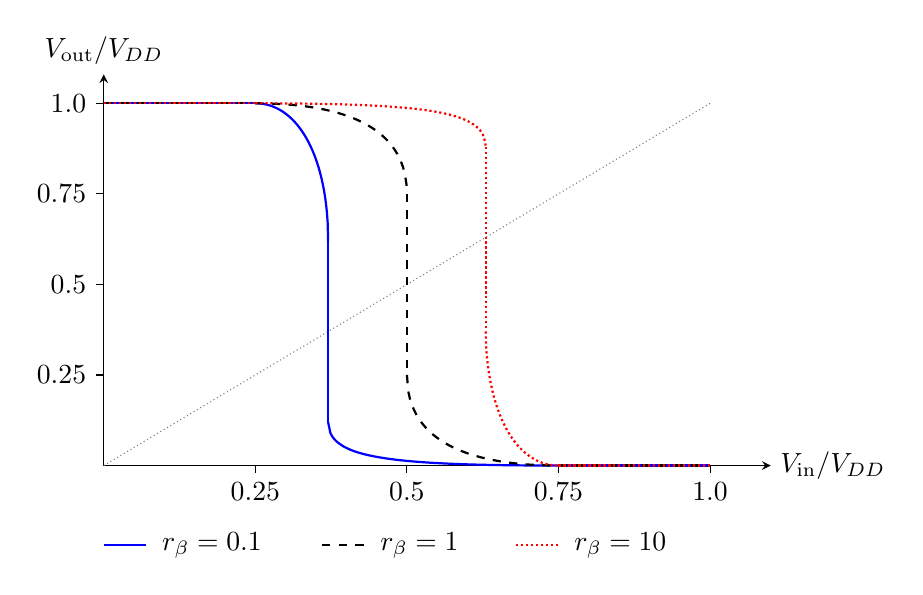
\begin{tikzpicture}[x=7.7cm,y=4.6cm,>=stealth,
 lowratio/.style={blue,thick},
 balancedratio/.style={black,thick,dashed},
 highratio/.style={red,thick,densely dotted}]
\draw[->] (0,0)--(1.10,0) node[right] {\(V_{\mathrm{in}}/V_{DD}\)};
\draw[->] (0,0)--(0,1.08) node[above] {\(V_{\mathrm{out}}/V_{DD}\)};
\foreach \x in {0.25,0.5,0.75,1.0}
 {\draw (\x,0)--(\x,-0.02) node[below] {\(\x\)};}
\foreach \y in {0.25,0.5,0.75,1.0}
 {\draw (0,\y)--(-0.013,\y) node[left] {\(\y\)};}
\draw[densely dotted,gray] (0,0)--(1,1);
\foreach \r/\curvestyle in {0.1/lowratio,1/balancedratio,10/highratio} {
 \pgfmathsetmacro{\m}{(0.25+sqrt(\r)*0.75)/(1+sqrt(\r))}
 \draw[\curvestyle] (0,1)--(0.25,1);
 \draw[\curvestyle,domain=0.25:\m,samples=100]
  plot (\x,{\x+0.25+sqrt(max(0,(0.75-\x)^2-(\x-0.25)^2/\r))})
  -- (\m,{\m+0.25});
 \draw[\curvestyle] (\m,{\m+0.25})--(\m,{\m-0.25});
 \draw[\curvestyle,domain=\m:0.75,samples=100]
  plot (\x,{\x-0.25-sqrt(max(0,(\x-0.25)^2-\r*(0.75-\x)^2))});
 \draw[\curvestyle] (0.75,0)--(1,0);
}
\draw[blue,thick] (0,-0.22)--(0.07,-0.22);
\node[anchor=west] at (0.08,-0.22) {\(r_\beta=0.1\)};
\draw[black,thick,dashed] (0.36,-0.22)--(0.43,-0.22);
\node[anchor=west] at (0.44,-0.22) {\(r_\beta=1\)};
\draw[red,thick,densely dotted] (0.68,-0.22)--(0.75,-0.22);
\node[anchor=west] at (0.76,-0.22) {\(r_\beta=10\)};
\end{tikzpicture}
\end{latin}
\caption{جابه‌جایی مشخصه انتقال با تغییر نسبت \lr{Beta} در مدل
مربعی ایده‌آل. محورها بی‌بعدند و خط مورب شرط
\(V_{\mathrm{out}}=V_{\mathrm{in}}\) را مشخص می‌کند.}
\label{fig:beta-vtc-family}
\end{figure}

\subsubsection{استخراج آستانه در حد \lr{Velocity Saturation}}
\label{sec:beta-velocity-limit}
در حد اشباع کامل سرعت، رابطه \secnum{۲.۲۹} کتاب جریان اشباع
را تقریباً متناسب با توان اول اضافه‌ولتاژ می‌دهد. با تعریف
\(K_n=W_nC_{\mathrm{ox},n}v_{\mathrm{sat},n}\) و
\(K_p=W_pC_{\mathrm{ox},p}v_{\mathrm{sat},p}\)، بزرگی دو جریان
رابطه \secnum{۲.۵۶} کتاب چنین نوشته می‌شود
\begin{equation}
 I_n=K_n(M-L),\qquad I_p=K_p(H-M).
 \label{eq:beta-velocity-currents}
\end{equation}
واحد \(K\) از حاصل‌ضرب
\(\mathrm{m}\times\mathrm{F\,m^{-2}}\times\mathrm{m\,s^{-1}}\)
برابر \(\mathrm{F\,s^{-1}}=\mathrm{A\,V^{-1}}\) است.
پس ضرب آن در ولتاژ، جریان می‌دهد.
این حد وقتی قابل استفاده است که محدودیت سرعت غالب باشد.
در \NotesTopic{sec:high-field}{مدل میدان قوی}، شرط متناظر
\(V_c\ll V_{GT}\) است و باید برای هر افزاره بررسی شود.

نسبت قدرت در این مدل را با نماد متمایز تعریف می‌کنیم
\begin{equation}
 \boxed{r_v=\frac{K_p}{K_n}
 =\frac{W_pC_{\mathrm{ox},p}v_{\mathrm{sat},p}}
        {W_nC_{\mathrm{ox},n}v_{\mathrm{sat},n}}}>0.
 \label{eq:beta-velocity-ratio}
\end{equation}
در فرض عایق گیت یکسان، \(C_{\mathrm{ox}}\) حذف می‌شود و همان
تعریف \(r=W_pv_{\mathrm{sat},p}/(W_nv_{\mathrm{sat},n})\)
صفحه ۹۰ کتاب به دست می‌آید. کتاب نماد \(r\) را در این مرحله
دوباره تعریف می‌کند. این جزوه از \(r_\beta\) و \(r_v\) استفاده
می‌کند تا مدل هر نسبت روشن باشد.

با برابرکردن جریان‌ها و تقسیم بر \(K_n>0\)، مراحل حل عبارت‌اند از
\begin{align}
 M-L&=r_v(H-M),\notag\\
 M+r_vM&=L+r_vH,\notag\\
 \boxed{M=\frac{L+r_vH}{1+r_v}
 =\frac{V_{tn}+r_v(V_{DD}-V_{TP})}{1+r_v}}.
 \label{eq:beta-velocity-threshold}
\end{align}
با تقسیم صورت و مخرج بر \(r_v\)، شکل رابطه \secnum{۲.۵۷}
کتاب حاصل می‌شود
\begin{equation}
 M=\frac{V_{DD}+V_{tp}+V_{tn}/r_v}{1+1/r_v}.
 \label{eq:beta-book-velocity-form}
\end{equation}
شرط دامنه نیز با
\(M-L=r_v\Delta/(1+r_v)>0\) و
\(H-M=\Delta/(1+r_v)>0\) تأیید می‌شود.
در \(r_v=1\) و آستانه‌های برابر، دوباره
\(M=V_{DD}/2\) است.

\paragraph*{مثال آموزشی مدل خطی اضافه‌ولتاژ}
فرض کنید حد اشباع کامل سرعت برای هر دو افزاره برقرار باشد،
\(V_{DD}=\qty{1.2}{\volt}\)،
\(V_{tn}=V_{TP}=\qty{0.3}{\volt}\)،
\(K_n=\qty{50}{\micro\ampere\per\volt}\) و
\(K_p=\qty{200}{\micro\ampere\per\volt}\).
این پارامترها یک مدل آموزشی مستقل را تعریف می‌کنند.
در \(r_v=4\)، داریم
\begin{equation*}
 M=\frac{0.3+4(0.9)}{5}=\qty{0.78}{\volt}.
\end{equation*}
اضافه‌ولتاژها \(\qty{0.48}{\volt}\) و \(\qty{0.12}{\volt}\) هستند.
برابری جریان‌ها با جای‌گذاری این دو مقدار کنترل می‌شود.
\[
 50(0.48)=200(0.12)=\qty{24}{\micro\ampere}.
\]
ولتاژهای \(V_{DS,n}=\qty{0.78}{\volt}\) و
\(V_{SD,p}=\qty{0.42}{\volt}\) از اضافه‌ولتاژهای متناظر بیشترند.
فرض محدودیت غالب سرعت، بخشی از مدل این مثال است.
تأیید آن در یک فناوری به پارامترهای \(V_c\) همان فناوری نیاز دارد.

\subsubsection{مقایسه حساسیت دو مدل و طراحی ابعاد}
\label{sec:beta-sensitivity-sizing}
جدول \ref{tab:beta-threshold-comparison} آستانه را با
\(L=\qty{0.3}{\volt}\) و \(H=\qty{0.9}{\volt}\) مقایسه می‌کند.
عدد نسبت در هر ستون، با تعریف همان مدل به کار رفته است.
قرارگرفتن دو مقدار برابر در یک ردیف، انتخاب آموزشی وزن‌های
بی‌بعد است. برای یک هندسه مشخص، باید هر نسبت جداگانه از
پارامترهای همان مدل محاسبه شود.
\begin{table}[!htbp]
\centering
\small
\caption{آستانه محاسبه‌شده از دو مدل برای نسبت‌های فرضی.
هر دو ستون آستانه برحسب \(\unit{\volt}\) هستند.}
\label{tab:beta-threshold-comparison}
\begin{tabular}{ccc}
\toprule
مقدار نسبت در مدل مربوط & \(M(r_\beta)\)، مدل مربعی & \(M(r_v)\)، حد سرعت\\
\midrule
\num{0.1} & \num{0.4442} & \num{0.3545}\\
\num{0.5} & \num{0.5485} & \num{0.5000}\\
\num{1} & \num{0.6000} & \num{0.6000}\\
\num{2} & \num{0.6515} & \num{0.7000}\\
\num{4} & \num{0.7000} & \num{0.7800}\\
\num{10} & \num{0.7558} & \num{0.8455}\\
\bottomrule
\end{tabular}
\end{table}

\paragraph*{استخراج حساسیت نزدیک نسبت یک}
مشتق \(\mathrm{d}M/\mathrm{d}r\)، تغییر آستانه در برابر تغییر
کوچک نسبت را اندازه می‌گیرد. برای مدل مربعی،
\(M=L+\Delta s/(1+s)\) و \(s=\sqrt{r_\beta}\) است.
مشتق \(s/(1+s)\) نسبت به \(s\) و مشتق ریشه به‌ترتیب چنین‌اند.
\[
 \frac{(1+s)-s}{(1+s)^2}=\frac{1}{(1+s)^2},\qquad
 \frac{\mathrm{d}s}{\mathrm{d}r_\beta}=\frac{1}{2\sqrt{r_\beta}}.
\]
با ضرب این دو نرخ، نتیجه می‌شود
\begin{equation}
 \frac{\mathrm{d}M}{\mathrm{d}r_\beta}
 =\frac{\Delta}{2\sqrt{r_\beta}(1+\sqrt{r_\beta})^2},\qquad
 \left.\frac{\mathrm{d}M}{\mathrm{d}r_\beta}\right|_{r_\beta=1}
 =\frac{\Delta}{8}.
 \label{eq:beta-long-sensitivity}
\end{equation}
برای مدل حد سرعت، \(M=L+\Delta r_v/(1+r_v)\) است، پس
\begin{equation}
 \frac{\mathrm{d}M}{\mathrm{d}r_v}
 =\frac{\Delta}{(1+r_v)^2},\qquad
 \left.\frac{\mathrm{d}M}{\mathrm{d}r_v}\right|_{r_v=1}
 =\frac{\Delta}{4}.
 \label{eq:beta-velocity-sensitivity}
\end{equation}
هر دو مشتق مثبت و دارای واحد ولت‌اند، زیرا نسبت بی‌بعد است.
در مقایسه حول نسبت یک و برای \(\Delta\) یکسان، حساسیت حد سرعت
دو برابر حساسیت مدل مربعی است. با \(\Delta=\qty{0.6}{\volt}\)،
شیب‌ها \(\qty{0.075}{\volt}\) و \(\qty{0.15}{\volt}\) به ازای
یک واحد تغییر نسبت‌اند. برای افزایش نسبت از یک به \num{1.1}،
تقریب خطی به‌ترتیب جابه‌جایی \(\qty{7.5}{\milli\volt}\) و
\(\qty{15}{\milli\volt}\) می‌دهد. محاسبه دقیق،
\(\qty{7.147}{\milli\volt}\) و
\(\qty{14.286}{\milli\volt}\) است.

مرجع حساسیت بیشتر مدارهای با محدودیت سرعت به \lr{Skew} را بیان
می‌کند \cite[پایان صفحه ۹۰]{weste}. مشتق‌های حاضر، این موضوع
را برای آستانه و نسبت‌های تعریف‌شده کمی می‌کنند.
شیب منحنی انتقال نسبت به ورودی، کمیت دیگری است و از
\eqref{eq:inverter-gain} و رسانایی‌های خروجی اثر می‌گیرد.
هر دو مدل ایده‌آل اشباع در استخراج آستانه، مستقل از خروجی‌اند و
در ناحیه اشباع هم‌زمان، گذار عمودی دارند. برای توصیف شیب محدود
مدار واقعی باید اثرهایی مانند \lr{CLM} نیز وارد شوند.

\paragraph*{از نسبت قدرت تا نسبت عرض}
رابطه هندسی مدل مربعی به صورت زیر است
\begin{equation}
 r_\beta=\frac{\mu_pC_{\mathrm{ox},p}}{\mu_nC_{\mathrm{ox},n}}
          \frac{W_p/L_p}{W_n/L_n}.
 \label{eq:beta-geometry-ratio}
\end{equation}
در طول و عایق یکسان،
\(r_\beta=(\mu_p/\mu_n)(W_p/W_n)\).
برای مثال فرضی \(\mu_p=0.5\mu_n\)، نسبت عرض دو،
\(r_\beta=1\) و نسبت عرض هشت، \(r_\beta=4\) می‌دهد.
کتاب معمولاً تغییر عرض با نگه‌داشتن طول کمینه مناسب فناوری را
برای تنظیم \lr{Skew} مطرح می‌کند \cite[صفحه ۹۰]{weste}.
تغییر طول هم‌زمان بر جریان، ظرفیت و اثرهای کانال کوتاه اثر دارد.
مقادیر ابعاد باید با تعریف ابعاد مؤثر مدل سازگار باشند.

در حد سرعت و با عایق یکسان،
\(r_v=(v_{\mathrm{sat},p}/v_{\mathrm{sat},n})(W_p/W_n)\).
اگر به‌طور آموزشی \(v_{\mathrm{sat},p}=0.8v_{\mathrm{sat},n}\)
و \(W_p/W_n=2\) فرض شوند، \(r_v=1.6\) است.
با \(\mu_p/\mu_n=0.5\)، همین نسبت عرض در مدل مربعی
\(r_\beta=1\) داشت. برای آستانه‌های \(\qty{0.3}{\volt}\) و
تغذیه \(\qty{1.2}{\volt}\)، نتیجه رسمی مدل مربعی
\(M=\qty{0.6}{\volt}\) است. محاسبه در حد سرعت می‌دهد
\[
 M=\frac{0.3+1.6\times0.9}{2.6}\approx\qty{0.6692}{\volt}.
\]
برای کاربرد هر حد باید دامنه اعتبار آن بررسی شود.

\paragraph*{طراحی معکوس برای آستانه مطلوب}
اگر آستانه هدف \(M_\star\) در \(L<M_\star<H\) باشد، از
\eqref{eq:beta-positive-root} و مدل حد سرعت به دست می‌آید
\begin{equation}
 \boxed{r_\beta=\left(\frac{M_\star-L}{H-M_\star}\right)^2},\qquad
 \boxed{r_v=\frac{M_\star-L}{H-M_\star}}.
 \label{eq:beta-inverse-sizing}
\end{equation}
هر دو کسر بی‌بعد و مثبت‌اند. نزدیک‌شدن هدف به \(H\)، مخرج را
کوچک و نسبت مورد نیاز را بزرگ می‌کند.
برای \(M_\star=\qty{0.65}{\volt}\)، \(L=\qty{0.3}{\volt}\)
و \(H=\qty{0.9}{\volt}\)، نسبت اضافه‌ولتاژها چنین محاسبه می‌شود.
\[
 \frac{0.65-0.3}{0.9-0.65}=\frac{0.35}{0.25}=1.4.
\]
پس \(r_\beta=1.96\) و \(r_v=1.4\) لازم است.
در مدل مربعی با \(\mu_p/\mu_n=0.5\)، طول و عایق یکسان،
نسبت عرض‌ها به دست می‌آید.
\[
 \frac{W_p}{W_n}=\frac{1.96}{0.5}=3.92.
\]
اگر \(W_n=\qty{0.4}{\micro\metre}\)،
\(W_p=\qty{1.568}{\micro\metre}\) خواهد بود.
این ابعاد، نتیجه مدل آموزشی‌اند و گردکردن ابعاد واقعی تابع قواعد
فناوری است. افزایش عرض، ظرفیت و مساحت را هم تغییر می‌دهد.

\subsubsection{تبدیل گیت‌های دیگر به \lr{Equivalent Inverter}}
\label{sec:beta-equivalent-inverter}
انتهای بخش \secnum{۲.۵.۲} کتاب و اسلاید ۸، تحلیل گیت‌های دیگر
با یک \lr{Equivalent Inverter} را مطرح می‌کنند
\cite[صفحه ۹۰ و آغاز ۹۱]{weste}\cite[اسلاید ۸]{dcslides}.
ابتدا ورودی‌های ثابت و متغیر و مسیرهای روشن را مشخص می‌کنیم.
چند ترانزیستور موازی روشن با بایاس‌های یکسان، جریان‌هایشان را جمع
می‌کنند و در مدل ساده، عرض مؤثر بیشتری می‌دهند. اگر تنها یک
شاخه موازی روشن باشد، شاخه‌های خاموش در جریان هدایت ایده‌آل
سهم صفر دارند. ظرفیت و نشتی آن شاخه‌ها در تحلیل‌های مربوط به
خود همچنان مطرح‌اند.

برای افزاره‌های یکسان موازی با گیت مشترک،
\(\beta_{\mathrm{eq}}=m\beta\) است که \(m\) تعداد واحدهای روشن
است. برای \(m\) واحد یکسان سری با گیت مشترک، در مدل
\lr{Shockley} با آستانه ثابت و بدون اثر بدنه و \lr{CLM}،
معادل طول \(mL_n\) یا \(mL_p\) و ضریب
\(\beta_{\mathrm{eq}}=\beta/m\) به کار می‌رود.
این نتیجه با برابری جریان‌ها و جمع افت ولتاژهای کانال سازگار است.
در مدل‌های غیرایده‌آل، به‌ویژه با اثر بدنه و محدودیت سرعت،
باید ناحیه کاری و گره‌های داخلی دوباره بررسی شوند.

\paragraph*{پیش‌نیاز \lr{NAND} و \lr{NOR}}
گیت دوورودی \lr{NAND}، متمم \lr{AND} است. خروجی فقط وقتی
صفر می‌شود که هر دو ورودی یک باشند. گیت \lr{NOR}، متمم
\lr{OR} است و خروجی فقط وقتی یک می‌شود که هر دو ورودی صفر
باشند. در پیاده‌سازی \lr{Static CMOS}، \lr{NAND} دو
\lr{nMOS} سری در شبکه پایین‌کش و دو \lr{pMOS} موازی در
شبکه بالاکش دارد. \lr{NOR} دو \lr{nMOS} موازی و دو
\lr{pMOS} سری دارد \cite[فصل ۱، بخش \secnum{۱.۴}]{weste}.
در مثال آموزشی حاضر، دو ورودی هر گیت به یک ولتاژ مشترک
\(v\) وصل می‌شوند تا مشخصه \(y(v)\) تک‌ورودی تعریف شود.

فرض کنید همه \lr{nMOS}ها ضریب \(\beta_n\) و همه
\lr{pMOS}ها ضریب \(\beta_p\) داشته باشند. با مدل سری و
موازی بیان‌شده، جدول \ref{tab:beta-equivalent-gates} حاصل می‌شود.
\begin{table}[!htbp]
\centering
\small
\caption{معادل آموزشی گیت‌ها با هر دو ورودی متصل به \(v\).
اثر بدنه، نشتی و \lr{CLM} صفر و آستانه‌ها ثابت‌اند.}
\label{tab:beta-equivalent-gates}
\begin{tabular}{cccc}
\toprule
گیت & \(\beta_{n,\mathrm{eq}}\) & \(\beta_{p,\mathrm{eq}}\) & نسبت معادل\\
\midrule
\lr{Inverter} & \(\beta_n\) & \(\beta_p\) & \(r_\beta\)\\
\lr{NAND} دوورودی & \(\beta_n/2\) & \(2\beta_p\) & \(4r_\beta\)\\
\lr{NOR} دوورودی & \(2\beta_n\) & \(\beta_p/2\) & \(r_\beta/4\)\\
\bottomrule
\end{tabular}
\end{table}
برای نمونه فرضی با \(r_\beta=1\)،
\(V_{tn}=V_{TP}=\qty{0.3}{\volt}\) و
\(V_{DD}=\qty{1.2}{\volt}\)، نسبت \lr{NAND} برابر چهار و
آستانه آن \(\qty{0.7}{\volt}\) است.
نسبت \lr{NOR} برابر \num{0.25} است. آستانه آن از رابطه مدل محاسبه می‌شود.
\[
 \frac{0.3+0.5\times0.9}{1.5}=\qty{0.5}{\volt}.
\]
این مقایسه به اتصال هر دو ورودی به \(v\) و فرض‌های مدل وابسته
است. وقتی یک ورودی ثابت و دیگری متغیر باشد، ولتاژ گیت‌های
افزاره‌های سری یکسان نیست و معادل ساده باید با تحلیل مدار
همان حالت ارزیابی شود.

\subsubsection{تمرین‌های تشریحی و کنترل نهایی}
\label{sec:beta-practice}
\paragraph*{تمرین آموزشی ۱ و آستانه‌های نابرابر}
با \(V_{DD}=\qty{1.2}{\volt}\)،
\(V_{tn}=\qty{0.35}{\volt}\)،
\(V_{TP}=\qty{0.25}{\volt}\) و \(r_\beta=4\)، آستانه
ورودی را در مدل مربعی حساب کنید.

\textbf{پاسخ.}
\(L=\qty{0.35}{\volt}\)، \(H=\qty{0.95}{\volt}\) و
\(s=2\) هستند. بنابراین،
\[
 M=\frac{0.35+2\times0.95}{3}=\qty{0.75}{\volt}.
\]
اضافه‌ولتاژها \(\qty{0.4}{\volt}\) و
\(\qty{0.2}{\volt}\) می‌شوند و نسبت مربع آن‌ها چهار است.
در \(y=M\)، \(V_{DS,n}=\qty{0.75}{\volt}\) و
\(V_{SD,p}=\qty{0.45}{\volt}\) از اضافه‌ولتاژها بیشترند.
پس هر دو شرط اشباع برقرار و \lr{KCL} سازگار است.

\paragraph*{تمرین آموزشی ۲ و یک نسبت از دو کمیت متفاوت}
فرض کنید \(\beta_p/\beta_n=4\). آیا می‌توان همین عدد را در
رابطه \eqref{eq:beta-velocity-threshold} گذاشت؟

\textbf{پاسخ.}
رابطه مذکور به \(r_v=K_p/K_n\) نیاز دارد. مقدار آن از
عرض‌ها، \(C_{\mathrm{ox}}\) و سرعت‌های اشباع به دست می‌آید.
برای نمونه با عایق و طول یکسان،
\(\mu_p/\mu_n=0.5\) و \(W_p/W_n=8\)،
\(r_\beta=4\) می‌شود. اگر
\(v_{\mathrm{sat},p}/v_{\mathrm{sat},n}=0.8\) هم فرض شود،
\(r_v=6.4\) است. برای \(L=\qty{0.3}{\volt}\) و
\(H=\qty{0.9}{\volt}\)، محاسبه در حد سرعت می‌دهد
\[
 M=\frac{0.3+6.4\times0.9}{7.4}\approx\qty{0.8189}{\volt}.
\]
اعتبار حد سرعت باید برای افزاره‌های مسئله برقرار باشد.

\paragraph*{تمرین آموزشی ۳ و بررسی هدف طراحی}
برای \(L=\qty{0.3}{\volt}\) و \(H=\qty{0.9}{\volt}\)،
هدف \(M_\star=\qty{0.95}{\volt}\) را بررسی کنید.

\textbf{پاسخ.}
هدف از \(H\) بیشتر است. در آن ورودی، افزاره \lr{pMOS} در
مدل هدایت قوی خاموش است و فرض استخراج اشباع هم‌زمان برقرار
نیست. رابطه میانگین وزنی \eqref{eq:beta-long-threshold} برای
نسبت مثبت، جواب را در \(L<M<H\) قرار می‌دهد.
پس این هدف با تغییر نسبت مثبت در همین مدل قابل دستیابی نیست.
مربع‌کردن کسر منفی در فرمول معکوس، شرط دامنه را برطرف نمی‌کند.

بخش \secnum{۲.۵.۳}، ارتباط مشخصه انتقال با بازه‌های معتبر
منطقی و تحمل نویز را بررسی می‌کند.

% !TeX root = booklet-03.tex
\clearpage
\subsection{سطوح منطقی و \lr{Noise Margin}}
\label{sec:noise-margin}
خروجی یک گیت، ورودی گیت بعدی را تغذیه می‌کند. برای انتقال صحیح
داده، بازه ولتاژ تولیدشده در خروجی باید در بازه معتبر ورودی گیت
گیرنده قرار گیرد. نویز می‌تواند ولتاژ دریافتی را تغییر دهد.
\lr{Noise Margin} مقدار تغییر نامطلوبی را توصیف می‌کند که این
سازگاری را در شرایط تعریف‌شده حفظ می‌کند
\cite[بخش \secnum{۲.۵.۳}، صفحات ۹۱ و ۹۲]{weste}
\cite[اسلایدهای ۹ و ۱۰]{dcslides}.

\subsubsection{تعریف چهار سطح ولتاژ}
\label{sec:noise-logic-levels}
برای ورودی، \(V_{\mathrm{IL}}\) بیشترین ولتاژ پذیرفته‌شده به‌عنوان
\lr{LOW} و \(V_{\mathrm{IH}}\) کمترین ولتاژ پذیرفته‌شده به‌عنوان
\lr{HIGH} است. برای خروجی، \(V_{\mathrm{OL}}\) بیشترین ولتاژ
تولیدشده در حالت \lr{LOW} و \(V_{\mathrm{OH}}\) کمترین ولتاژ
تولیدشده در حالت \lr{HIGH} است. حرف \lr{I} به ورودی، حرف
\lr{O} به خروجی و حرف‌های \lr{L} و \lr{H} به سطح پایین و بالا
اشاره می‌کنند. جدول \ref{tab:noise-level-definitions} تعریف‌ها
را به شکل بازه نشان می‌دهد \cite[صفحه ۹۱]{weste}.
\begin{table}[!htbp]
\centering
\small
\caption{بازه‌های منطقی برای ولتاژهای بین زمین و تغذیه.
مرزهای ورودی به گیرنده و مرزهای خروجی به فرستنده مربوط‌اند.}
\label{tab:noise-level-definitions}
\begin{tabularx}{\linewidth}{cc>{\raggedleft\arraybackslash}X}
\toprule
پایانه & حالت & بازه معتبر\\
\midrule
ورودی & \lr{LOW} & \(0\le V_{\mathrm{in}}\le V_{\mathrm{IL}}\)\\
ورودی & \lr{HIGH} & \(V_{\mathrm{IH}}\le V_{\mathrm{in}}\le V_{DD}\)\\
خروجی & \lr{LOW} & \(0\le V_{\mathrm{out}}\le V_{\mathrm{OL}}\)\\
خروجی & \lr{HIGH} & \(V_{\mathrm{OH}}\le V_{\mathrm{out}}\le V_{DD}\)\\
\bottomrule
\end{tabularx}
\end{table}

بازه \(V_{\mathrm{IL}}<V_{\mathrm{in}}<V_{\mathrm{IH}}\) را
\lr{Indeterminate Region} یا \lr{Forbidden Zone} می‌نامند.
در این بازه، مشخصات منطقیِ تعریف‌شده، تفسیر معتبر صفر یا یک را
تضمین نمی‌کنند. مدار همچنان ولتاژ و جریان فیزیکی دارد و می‌توان
آن را با مشخصه انتقال تحلیل کرد.
\(V_{\mathrm{inv}}\) نیز نقطه \(V_{\mathrm{out}}=V_{\mathrm{in}}\)
از بخش \ref{sec:inverter-input-threshold} است. دو مرز
\(V_{\mathrm{IL}},V_{\mathrm{IH}}\) با معیار جداگانه‌ای تعیین
می‌شوند که در ادامه استخراج می‌شود.

در شرایط سازگار معمول، خروجی پایین باید از حداکثر ورودی پایین
کمتر و خروجی بالا باید از حداقل ورودی بالا بیشتر باشد. شکل
\ref{fig:noise-level-ranges} فاصله‌های مربوط را نشان می‌دهد.
\begin{figure}[!htbp]
\centering
\begin{latin}
\PersianMathDigits
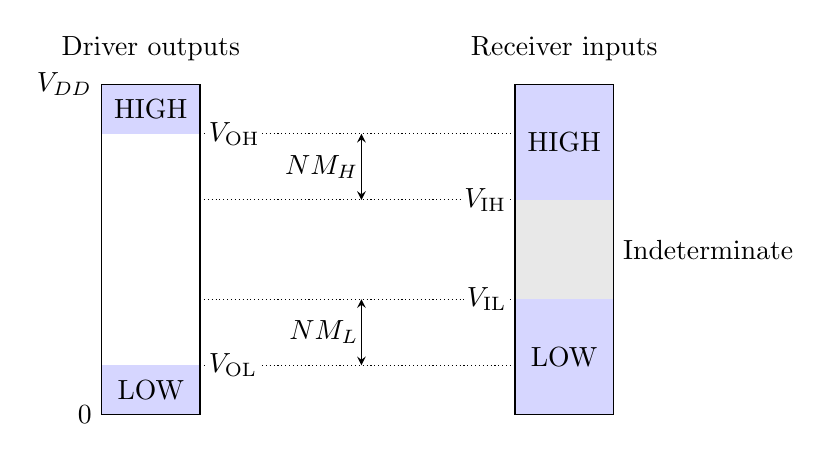
\begin{tikzpicture}[x=1cm,y=4.2cm,>=stealth]
\fill[blue!16] (0,0) rectangle (1.25,0.15);
\fill[blue!16] (0,0.85) rectangle (1.25,1);
\draw (0,0) rectangle (1.25,1);
\fill[blue!16] (5.25,0) rectangle (6.5,0.35);
\fill[gray!18] (5.25,0.35) rectangle (6.5,0.65);
\fill[blue!16] (5.25,0.65) rectangle (6.5,1);
\draw (5.25,0) rectangle (6.5,1);
\foreach \y in {0.15,0.35,0.65,0.85}
 {\draw[densely dotted] (1.25,\y)--(5.25,\y);}
\node[above] at (0.625,1.04) {Driver outputs};
\node[above] at (5.875,1.04) {Receiver inputs};
\node[left] at (0,0) {\(0\)};
\node[left] at (0,1) {\(V_{DD}\)};
\node at (0.625,0.075) {LOW};
\node at (0.625,0.925) {HIGH};
\node at (5.875,0.175) {LOW};
\node at (5.875,0.825) {HIGH};
\node[right] at (6.5,0.5) {Indeterminate};
\node[anchor=west,fill=white,inner sep=1pt] at (1.32,0.15) {\(V_{\mathrm{OL}}\)};
\node[anchor=west,fill=white,inner sep=1pt] at (1.32,0.85) {\(V_{\mathrm{OH}}\)};
\node[anchor=east,fill=white,inner sep=1pt] at (5.18,0.35) {\(V_{\mathrm{IL}}\)};
\node[anchor=east,fill=white,inner sep=1pt] at (5.18,0.65) {\(V_{\mathrm{IH}}\)};
\draw[<->] (3.3,0.15)--(3.3,0.35)
 node[midway,left,fill=white,inner sep=1pt] {\(NM_L\)};
\draw[<->] (3.3,0.65)--(3.3,0.85)
 node[midway,left,fill=white,inner sep=1pt] {\(NM_H\)};
\end{tikzpicture}
\end{latin}
\caption{طرح آموزشی بازه‌های ورودی و خروجی بر اساس شکل
\secnum{۲.۲۹} کتاب و اسلاید ۹. فاصله‌ها شماتیک‌اند و مقیاس
عددی یک فناوری را نمایش نمی‌دهند.}
\label{fig:noise-level-ranges}
\end{figure}

\subsubsection{استخراج حاشیه نویز از شرط سازگاری}
\label{sec:noise-margin-definition}
برای حالت پایین، بدترین خروجی مجاز فرستنده
\(V_{\mathrm{OL}}\) است. اگر نویز نامطلوب مثبت با بزرگی
\(v_n\ge0\) به آن اضافه شود، ولتاژ دریافتی در این حالت
\(V_{\mathrm{OL}}+v_n\) می‌شود. برای باقی‌ماندن در بازه
\lr{LOW} گیرنده، باید
\begin{equation*}
 V_{\mathrm{OL}}+v_n\le V_{\mathrm{IL}}
 \quad\Longrightarrow\quad
 v_n\le V_{\mathrm{IL}}-V_{\mathrm{OL}}.
\end{equation*}
پس رابطه \secnum{۲.۵۸} کتاب چنین تعریف می‌شود
\begin{equation}
 \boxed{NM_L=V_{\mathrm{IL}}-V_{\mathrm{OL}}}.
 \label{eq:noise-low-margin}
\end{equation}
برای حالت بالا، بدترین خروجی مجاز
\(V_{\mathrm{OH}}\) است. نویز نامطلوب، ولتاژ را کاهش می‌دهد.
شرط باقی‌ماندن ورودی در بازه \lr{HIGH} برابر است با
\begin{equation*}
 V_{\mathrm{OH}}-v_n\ge V_{\mathrm{IH}}
 \quad\Longrightarrow\quad
 v_n\le V_{\mathrm{OH}}-V_{\mathrm{IH}}.
\end{equation*}
در نتیجه، رابطه \secnum{۲.۵۹} کتاب چنین است
\begin{equation}
 \boxed{NM_H=V_{\mathrm{OH}}-V_{\mathrm{IH}}}.
 \label{eq:noise-high-margin}
\end{equation}
هر دو حاشیه واحد ولت دارند. وقتی بزرگی نویز در هر دو حالت
مهم باشد، کمیت \(\min(NM_L,NM_H)\) حاشیه محدودکننده را
نشان می‌دهد. مقدار صفر، فاصله اطمینان اضافی باقی نمی‌گذارد.
مقدار منفی یعنی حتی بدون نویز اضافه، همه خروجی‌های مجاز
فرستنده در بازه معتبر گیرنده قرار نمی‌گیرند.

\paragraph*{مثال آموزشی ارتباط دو گیت}
فرض کنید فرستنده \(V_{\mathrm{OL}}=\qty{0.1}{\volt}\) و
\(V_{\mathrm{OH}}=\qty{0.9}{\volt}\) و گیرنده
\(V_{\mathrm{IL}}=\qty{0.3}{\volt}\) و
\(V_{\mathrm{IH}}=\qty{0.7}{\volt}\) داشته باشند.
هر دو حاشیه \(\qty{0.2}{\volt}\) هستند.
نویز مثبت \(\qty{0.15}{\volt}\) روی بدترین سطح پایین،
ورودی \(\qty{0.25}{\volt}\) می‌دهد که هنوز معتبر است.
نویز کاهنده با همین بزرگی روی بدترین سطح بالا،
\(\qty{0.75}{\volt}\) می‌دهد که آن هم معتبر است.
اما با نویز مثبت \(\qty{0.25}{\volt}\)، سطح پایین به
\(\qty{0.35}{\volt}\) می‌رسد و وارد بازه نامعین می‌شود.
در این حالت، تضمین مشخصات منطقی از بین می‌رود. مقدار خروجی
واقعی باید از مشخصه گیرنده تعیین شود.

\subsubsection{معنای \lr{Unity Gain} و بدترین خروجی مجاز}
\label{sec:noise-unity-gain}
شیب مشخصه را با \(g\) نشان می‌دهیم. تعریف مشتق و تقریب تغییر کوچک
ورودی در همسایگی یک نقطه چنین‌اند.
\[
 g=\frac{\mathrm{d}V_{\mathrm{out}}}{\mathrm{d}V_{\mathrm{in}}},\qquad
 \Delta V_{\mathrm{out}}\approx g\Delta V_{\mathrm{in}}.
\]
مثلاً در \(g=-0.3\)، تغییر ورودی
\(\qty{10}{\milli\volt}\)، تقریباً
\(-\qty{3}{\milli\volt}\) تغییر خروجی ایجاد می‌کند.
در \(g=-4\)، همان تغییر ورودی حدود
\(-\qty{40}{\milli\volt}\) تغییر خروجی می‌دهد.
علامت منفی، رفتار معکوس‌کننده و بزرگی شیب، نسبت بزرگی تغییرها
را نشان می‌دهد.

نزدیک دو ریل، معمولاً \(|g|<1\) و در بخش میانی گذار،
\(|g|>1\) است. در قرارداد کتاب و اسلاید ۱۰، دو نقطه مرزی
با شرط زیر تعیین می‌شوند
\begin{equation}
 \boxed{g=-1}.
 \label{eq:noise-unity-condition}
\end{equation}
واژه \lr{Unity} به بزرگی یک اشاره دارد. چون مشخصه
\lr{Inverter} کاهشی است، مقدار علامت‌دار شیب منفی یک است.
نقطه سمت چپ، \(V_{\mathrm{IL}}\) و نقطه سمت راست،
\(V_{\mathrm{IH}}\) را مشخص می‌کند.
کتاب این مرزبندی را کرانی محافظه‌کارانه برای بدترین حاشیه نویز
ایستا توصیف می‌کند \cite[شکل \secnum{۲.۳۰} و صفحه ۹۲]{weste}.

در شاخه بالای یک مشخصه کاهشی، بیشترین ورودی پایین مجاز،
کمترین خروجی بالا را می‌دهد. در شاخه پایین، کمترین ورودی بالا
مجاز، بیشترین خروجی پایین را می‌دهد. بنابراین، برای همین
قرارداد سطوح منطقی می‌نویسیم
\begin{equation}
 V_{\mathrm{OH}}=V_{\mathrm{out}}(V_{\mathrm{IL}}),\qquad
 V_{\mathrm{OL}}=V_{\mathrm{out}}(V_{\mathrm{IH}}).
 \label{eq:noise-output-levels}
\end{equation}
در دو نقطه مرزی، خروجی می‌تواند کمی از ریل متناظر فاصله داشته
باشد. کتاب این انتقال اثر ورودی به خروجی را
\lr{Noise Feedthrough} یا \lr{Propagated Noise} می‌نامد
\cite[صفحه ۹۲]{weste}. این افت باید در تفاضل حاشیه‌ها لحاظ شود.

شکل \ref{fig:noise-unity-vtc} یک مثال آموزشی متقارن با
\(V_t=0.1V_{DD}\) است. روابط مدل مربعی بخش‌های قبل برای رسم
آن به کار رفته‌اند. در این مثال،
\(V_{\mathrm{IL}}=0.4V_{DD}\)،
\(V_{\mathrm{IH}}=0.6V_{DD}\)،
\(V_{\mathrm{OH}}=0.9V_{DD}\) و
\(V_{\mathrm{OL}}=0.1V_{DD}\) هستند.
\begin{figure}[!htbp]
\centering
\begin{latin}
\PersianMathDigits
\begin{tikzpicture}[x=8.4cm,y=5cm,>=stealth]
\draw[->] (0,0)--(1.1,0) node[right] {\(V_{\mathrm{in}}/V_{DD}\)};
\draw[->] (0,0)--(0,1.12) node[above] {\(V_{\mathrm{out}}/V_{DD}\)};
\draw[thick,blue] (0,1)--(0.1,1);
\draw[thick,blue,domain=0.1:0.5,samples=110]
 plot (\x,{\x+0.1+sqrt(max(0,(1-2*\x)*0.8))})--(0.5,0.6);
\draw[thick,blue] (0.5,0.6)--(0.5,0.4);
\draw[thick,blue,domain=0.5:0.9,samples=110]
 plot (\x,{\x-0.1-sqrt(max(0,(2*\x-1)*0.8))});
\draw[thick,blue] (0.9,0)--(1,0);
\draw[densely dotted] (0.4,0)--(0.4,0.9)--(0,0.9);
\draw[densely dotted] (0.6,0)--(0.6,0.1)--(0,0.1);
\draw[thick,red] (0.34,0.96)--(0.46,0.84);
\draw[thick,red] (0.54,0.16)--(0.66,0.04);
\fill (0.4,0.9) circle[radius=1.7pt];
\fill (0.6,0.1) circle[radius=1.7pt];
\node[below] at (0.4,0) {\(V_{\mathrm{IL}}/V_{DD}\)};
\node[below] at (0.6,0) {\(V_{\mathrm{IH}}/V_{DD}\)};
\node[below] at (1,0) {\(1\)};
\node[left] at (0,0.9) {\(V_{\mathrm{OH}}/V_{DD}\)};
\node[left] at (0,0.1) {\(V_{\mathrm{OL}}/V_{DD}\)};
\node[left] at (0,1) {\(1\)};
\node[above right] at (0.65,0.65) {\(g=-1\)};
\end{tikzpicture}
\end{latin}
\caption{نقاط \lr{Unity Gain} در مثال فرضی
\(V_t/V_{DD}=0.1\). پاره‌خط‌های قرمز مماس‌های با شیب منفی یک
در مختصات نرمال‌شده‌اند. ساخت شکل بر اساس شکل \secnum{۲.۳۰}
کتاب و اسلاید ۱۰ است.}
\label{fig:noise-unity-vtc}
\end{figure}

\subsubsection{پیش‌نیاز مشتق‌گیری و استخراج شیب دو شاخه}
\label{sec:noise-derivatives}
برای استخراج تحلیلی، مدل متقارن
\(\beta_n=\beta_p\)، \(V_{tn}=V_{TP}=V_t>0\) و
\(V_{DD}>2V_t\) را به کار می‌بریم. آستانه و \lr{Mobility}
ثابت و اثرهای نشتی و \lr{CLM} صفر فرض می‌شوند.
کمیت مثبت \(K=V_{DD}-2V_t\) را با واحد ولت تعریف می‌کنیم.
برای کوتاه‌شدن محاسبه، \(x=V_{\mathrm{in}}\) و
\(y=V_{\mathrm{out}}\) می‌گذاریم. روابط شاخه‌های \lr{B} و
\lr{D} از \eqref{eq:inverter-b-transfer} و
\eqref{eq:inverter-d-transfer} هستند.

مشتق یک مقدار ثابت نسبت به \(x\) صفر و مشتق خود \(x\) یک است.
برای ریشه، اگر \(z=\sqrt{u}>0\)، آنگاه \(z^2=u\).
مشتق‌گیری دو طرف نسبت به \(u\) می‌دهد
\[
 2z\frac{\mathrm{d}z}{\mathrm{d}u}=1
 \quad\Longrightarrow\quad
 \frac{\mathrm{d}\sqrt{u}}{\mathrm{d}u}=\frac{1}{2\sqrt{u}}.
\]
وقتی \(u\) خودش تابع \(x\) است، نرخ تغییر بیرونی را در نرخ
تغییر درونی ضرب می‌کنیم. این همان \lr{Chain Rule} است
\begin{equation}
 \frac{\mathrm{d}\sqrt{u(x)}}{\mathrm{d}x}
 =\frac{1}{2\sqrt{u(x)}}\frac{\mathrm{d}u}{\mathrm{d}x},
 \qquad u(x)>0.
 \label{eq:noise-chain-rule}
\end{equation}
این رابطه در شاخه‌های باز و دور از رادیکال صفر به کار می‌رود.

در شاخه \lr{B}، \(u(x)=K(V_{DD}-2x)\) و
\(\mathrm{d}u/\mathrm{d}x=-2K\) است. بنابراین،
\begin{align}
 y_B&=x+V_t+\sqrt{K(V_{DD}-2x)},\notag\\
 \frac{\mathrm{d}y_B}{\mathrm{d}x}
 &=1+\frac{-2K}{2\sqrt{K(V_{DD}-2x)}}\notag\\
 &=\boxed{1-\sqrt{\frac{K}{V_{DD}-2x}}}.
 \label{eq:noise-b-slope}
\end{align}
چون \(K>0\) و \(V_{DD}-2x>0\) در \lr{B}، تبدیل
\(K/\sqrt{K(V_{DD}-2x)}\) به ریشه نسبت، مجاز است.
نسبت داخل رادیکال بی‌بعد است، پس مشتق نیز بی‌بعد می‌شود.
شیب در ابتدای شاخه به صفر و هنگام نزدیک‌شدن به نقطه میانی
از چپ، به سمت مقادیر منفی با بزرگی زیاد می‌رود.

در شاخه \lr{D}، \(u(x)=K(2x-V_{DD})\) و
\(\mathrm{d}u/\mathrm{d}x=2K\) است. علامت منفی جلوی ریشه را
هم حفظ می‌کنیم
\begin{align}
 y_D&=x-V_t-\sqrt{K(2x-V_{DD})},\notag\\
 \frac{\mathrm{d}y_D}{\mathrm{d}x}
 &=1-\frac{2K}{2\sqrt{K(2x-V_{DD})}}\notag\\
 &=\boxed{1-\sqrt{\frac{K}{2x-V_{DD}}}}.
 \label{eq:noise-d-slope}
\end{align}
در این شاخه نیز رادیکال مثبت است. شیب از بزرگی زیاد نزدیک
گذار میانی به صفر در انتهای شاخه نزدیک می‌شود.

\subsubsection{استخراج چهار سطح در مدل متقارن}
\label{sec:noise-symmetric-levels}
با گذاشتن \(x=V_{\mathrm{IL}}\) و شیب منفی یک در
\eqref{eq:noise-b-slope}، داریم
\begin{align}
 1-\sqrt{\frac{K}{V_{DD}-2V_{\mathrm{IL}}}}&=-1,\notag\\
 \sqrt{\frac{K}{V_{DD}-2V_{\mathrm{IL}}}}&=2,\notag\\
 V_{DD}-2V_{\mathrm{IL}}&=\frac{K}{4},\notag\\
 \boxed{V_{\mathrm{IL}}=\frac{3V_{DD}+2V_t}{8}}.
 \label{eq:noise-vil}
\end{align}
ریشه سمت چپ مثبت است و برابر دو قرار داده شده است. با
مربع‌کردن، عدد چهار به دست می‌آید. حل سطر سوم و جای‌گذاری
\(K=V_{DD}-2V_t\)، سطر نهایی را می‌دهد.

با گذاشتن \(x=V_{\mathrm{IH}}\) در شاخه \lr{D}، به همین ترتیب
\begin{align}
 1-\sqrt{\frac{K}{2V_{\mathrm{IH}}-V_{DD}}}&=-1,\notag\\
 2V_{\mathrm{IH}}-V_{DD}&=\frac{K}{4},\notag\\
 \boxed{V_{\mathrm{IH}}=\frac{5V_{DD}-2V_t}{8}}.
 \label{eq:noise-vih}
\end{align}
برای کنترل دامنه، تفاضل با مرزهای شاخه را محاسبه می‌کنیم
\begin{align*}
 V_{\mathrm{IL}}-V_t
 &=V_{DD}-V_t-V_{\mathrm{IH}}=\frac{3K}{8}>0,\\
 \frac{V_{DD}}{2}-V_{\mathrm{IL}}
 &=V_{\mathrm{IH}}-\frac{V_{DD}}{2}=\frac{K}{8}>0.
\end{align*}
پس \(V_{\mathrm{IL}}\) واقعاً داخل \lr{B} و
\(V_{\mathrm{IH}}\) داخل \lr{D} است. هیچ‌یک روی پاره‌خط
عمودی ناحیه \lr{C} قرار ندارد.

در هر نقطه مرزی، مقدار رادیکال با شرط مثبت‌بودن \(K\) محاسبه می‌شود.
\[
 \sqrt{K(K/4)}=K/2,\qquad K>0.
\]
با استفاده از \eqref{eq:noise-output-levels}، سطوح خروجی به
دست می‌آیند
\begin{align}
 V_{\mathrm{OH}}&=V_{\mathrm{IL}}+V_t+\frac{K}{2}
 =\boxed{\frac{7V_{DD}+2V_t}{8}},\notag\\
 V_{\mathrm{OL}}&=V_{\mathrm{IH}}-V_t-\frac{K}{2}
 =\boxed{\frac{V_{DD}-2V_t}{8}}.
 \label{eq:noise-voh-vol}
\end{align}
بنابراین، افت خروجی در مرزهای ورودی مجاز چنین است.
\[
 V_{DD}-V_{\mathrm{OH}}=V_{\mathrm{OL}}=K/8.
\]
در این دامنه، افت مثبت است.
حاشیه‌ها با تفاضل سطوح محاسبه می‌شوند
\begin{align}
 NM_L&=\frac{3V_{DD}+2V_t}{8}-\frac{V_{DD}-2V_t}{8}
 =\frac{V_{DD}+2V_t}{4},\notag\\
 NM_H&=\frac{7V_{DD}+2V_t}{8}-\frac{5V_{DD}-2V_t}{8}
 =\frac{V_{DD}+2V_t}{4}.
 \label{eq:noise-symmetric-margins}
\end{align}
پس دو حاشیه برابرند. روابط
\(V_{\mathrm{IL}}+V_{\mathrm{IH}}=V_{DD}\) و
\(V_{\mathrm{OL}}+V_{\mathrm{OH}}=V_{DD}\) نیز تقارن را
تأیید می‌کنند. عرض بازه نامعین در این مدل برابر است با
\(V_{\mathrm{IH}}-V_{\mathrm{IL}}=K/4\).

\subsubsection{حل کامل تمرین \secnum{۲.۱۷}}
\label{sec:noise-ex17}
صورت اصلی تمرین، استفاده از نتایج تمرین \secnum{۲.۱۶} برای محاسبه
حاشیه نویز یک \lr{CMOS Inverter} با تغذیه
\(\qty{1.0}{\volt}\)، آستانه‌های
\(V_{tn}=|V_{tp}|=\qty{0.35}{\volt}\) و
\(\beta_n=\beta_p\) را می‌خواهد
\cite[تمرین \secnum{۲.۱۷}، صفحه چاپی ۹۷]{weste}.
روابط انتقال لازم پیش‌تر در بخش
\ref{sec:inverter-five-regions} استخراج شده‌اند.
همان مدل \lr{Shockley}، آستانه ثابت، بدنه متصل به سورس و
بار بدون جریان \lr{DC} را به کار می‌بریم. اثرهای نشتی و
\lr{CLM} در مدل این تمرین صفرند.

ابتدا پارامتر \(K\) را محاسبه و علامت آن را کنترل می‌کنیم.
\[
 K=1.0-2(0.35)=\qty{0.30}{\volt}>0.
\]
پس فرض وجود شاخه‌های \lr{B} و \lr{D} برقرار است.
با جای‌گذاری در روابط استخراج‌شده، داریم
\begin{align*}
 V_{\mathrm{IL}}&=\frac{3(1.0)+2(0.35)}{8}
 =\qty{0.4625}{\volt},\\
 V_{\mathrm{IH}}&=\frac{5(1.0)-2(0.35)}{8}
 =\qty{0.5375}{\volt},\\
 V_{\mathrm{OH}}&=\frac{7(1.0)+2(0.35)}{8}
 =\qty{0.9625}{\volt},\\
 V_{\mathrm{OL}}&=\frac{1.0-2(0.35)}{8}
 =\qty{0.0375}{\volt}.
\end{align*}
ارقام اعشاری برای بازبینی محاسبه مدل حفظ شده‌اند.
این تعداد رقم، دقت فیزیکی یک فناوری را تعیین نمی‌کند.
تفاضل‌های لازم می‌دهند
\begin{equation*}
 \boxed{NM_L=0.4625-0.0375=\qty{0.425}{\volt}},\qquad
 \boxed{NM_H=0.9625-0.5375=\qty{0.425}{\volt}}.
\end{equation*}
هر حاشیه \num{42.5} درصد تغذیه است.
در صورت گزارش با دو رقم اعشار و قاعده گردکردن نیم‌به‌بالا،
\(\qty{0.43}{\volt}\) حاصل می‌شود. محاسبه اصلی با مقادیر
گردنشده انجام می‌شود. اگر چهار سطح را ابتدا به دو رقم اعشار
گرد کنیم، تفاضل \(0.46-0.04=\qty{0.42}{\volt}\) به دست
می‌آید. این مثال اثر گردکردن میانی را نشان می‌دهد.

\paragraph*{کنترل جریان و ناحیه کاری در نقطه چپ}
در \(V_{\mathrm{in}}=\qty{0.4625}{\volt}\) و
\(V_{\mathrm{out}}=\qty{0.9625}{\volt}\)،
اضافه‌ولتاژها \(a=\qty{0.1125}{\volt}\) و
\(b=\qty{0.1875}{\volt}\) هستند.
\(V_{DS,n}=\qty{0.9625}{\volt}>a\)، پس \lr{nMOS} در
اشباع است. \(V_{SD,p}=\qty{0.0375}{\volt}<b\)، پس
\lr{pMOS} در \lr{Linear} است.
چون مقدار عددی \(\beta\) در صورت مسئله داده نشده است،
جریان‌ها را بر \(\beta\) تقسیم می‌کنیم
\begin{align}
 \frac{I_n}{\beta}&=\frac{(0.1125)^2}{2}
 =\qty{0.006328125}{\volt\squared},\notag\\
 \frac{I_p}{\beta}&=(0.1875)(0.0375)-\frac{(0.0375)^2}{2}
 =\qty{0.006328125}{\volt\squared}.
 \label{eq:noise-ex17-kcl}
\end{align}
واحد نسبت، آمپر تقسیم بر آمپر بر ولت مربع و برابر ولت مربع است.
برابری دو نسبت، \lr{KCL} را برای هر \(\beta>0\) تأیید می‌کند.
شیب نیز از \eqref{eq:noise-b-slope} به دست می‌آید.
\[
 1-\sqrt{\frac{0.30}{1-2\times0.4625}}=1-2=-1.
\]

\paragraph*{کنترل نقطه راست و حاشیه‌ها}
در \(V_{\mathrm{in}}=\qty{0.5375}{\volt}\)، خروجی
\(\qty{0.0375}{\volt}\)، اضافه‌ولتاژ \lr{nMOS}
\(\qty{0.1875}{\volt}\) و اضافه‌ولتاژ \lr{pMOS}
\(\qty{0.1125}{\volt}\) است.
بنابراین \lr{nMOS} در \lr{Linear} و \lr{pMOS} در اشباع
قرار می‌گیرند. دو نسبت جریان، همان مقدار
\eqref{eq:noise-ex17-kcl} را دارند. محاسبه شیب می‌دهد
\[
 1-\sqrt{\frac{0.30}{0.075}}=-1.
\]
همچنین ترتیب چهار سطح تأیید می‌شود.
\[
 0.0375<0.4625<0.5375<0.9625.
\]
در بدترین سطح پایین، افزودن
\(\qty{0.425}{\volt}\)، ورودی را دقیقاً به
\(\qty{0.4625}{\volt}\) می‌رساند.
در بدترین سطح بالا، کم‌کردن همین مقدار،
\(\qty{0.5375}{\volt}\) می‌دهد. هر دو، روی مرز مجاز قرار دارند.

\subsubsection{اثر \lr{Skew}، آستانه و مقیاس تغذیه}
\label{sec:noise-skew-tradeoff}
کتاب بیان می‌کند که در حالت متقارن، دو حاشیه برابرند و این
تعادل برای نویز با جهت نامشخص مطلوب است. اگر یک حالت منطقی
بیشتر در معرض نویز باشد، با \lr{Skew} می‌توان حاشیه آن را
بهبود داد و تغییر حاشیه دیگر را نیز باید پذیرفت
\cite[صفحه ۹۲]{weste}.

برای محاسبه در مدل مربعی نامتقارن، می‌توان از شاخه‌های
\eqref{eq:beta-b-transfer} و \eqref{eq:beta-d-transfer} استفاده
کرد. چون \(\mathrm{d}a/\mathrm{d}x=1\) و
\(\mathrm{d}b/\mathrm{d}x=-1\)، همان \lr{Chain Rule} می‌دهد
\begin{equation}
 g_B=1-\frac{b+a/r_\beta}{\sqrt{b^2-a^2/r_\beta}},\qquad
 g_D=1-\frac{a+r_\beta b}{\sqrt{a^2-r_\beta b^2}}.
 \label{eq:noise-skew-slopes}
\end{equation}
برای نمونه، مشتق رادیکال شاخه \lr{B} به صورت زیر نوشته می‌شود.
\[
 \frac{-2b-2a/r_\beta}{2\sqrt{b^2-a^2/r_\beta}}.
\]
در هر شاخه، ریشه \(g=-1\) را در دامنه همان شاخه پیدا
می‌کنیم، سپس خروجی‌های متناظر را محاسبه می‌کنیم.
جدول \ref{tab:noise-skew-example} نتیجه حل عددی این شرط را
برای سه نسبت فرضی، با تغذیه \(\qty{1}{\volt}\) و آستانه‌های
برابر \(\qty{0.35}{\volt}\)، نشان می‌دهد.
\begin{table}[!htbp]
\centering
\small
\caption{مقایسه حاشیه‌های مدل مربعی با \lr{Skew} فرضی.
همه ولتاژها برحسب \(\unit{\volt}\) و مقادیر تا چهار رقم اعشار گرد شده‌اند.}
\label{tab:noise-skew-example}
\begin{tabular}{cccccc}
\toprule
\(r_\beta\) & \(V_{\mathrm{IL}}\) & \(V_{\mathrm{IH}}\) &
\(NM_L\) & \(NM_H\) & کمترین حاشیه\\
\midrule
\num{0.5} & \num{0.4295} & \num{0.5036} & \num{0.3893} & \num{0.4657} & \num{0.3893}\\
\num{1} & \num{0.4625} & \num{0.5375} & \num{0.4250} & \num{0.4250} & \num{0.4250}\\
\num{2} & \num{0.4964} & \num{0.5705} & \num{0.4657} & \num{0.3893} & \num{0.3893}\\
\bottomrule
\end{tabular}
\end{table}
در این نمونه، تقویت \lr{pMOS}، حاشیه پایین را افزایش و حاشیه
بالا را کاهش داده است. \(NM_L\) به تحمل افزایش ولتاژ روی سطح
پایین مربوط است. \(NM_H\) به تحمل کاهش ولتاژ روی سطح بالا
مربوط می‌شود. انتخاب نسبت باید با نوع نویز و نیاز مدار سازگار باشد.
مقدارهای \(0.46V_{DD}\) و \(0.13V_{DD}\) نوشته‌شده در کنار
شکل \secnum{۲.۳۰} کتاب، به همان نمونه مرجع مربوط‌اند
\cite[صفحه ۹۲]{weste}.

در مدل متقارن \eqref{eq:noise-symmetric-margins}، با ثابت‌بودن
تغذیه، افزایش \(V_t\)، حاشیه‌ها را با نرخ
\(\mathrm{d}NM/\mathrm{d}V_t=1/2\) افزایش می‌دهد.
هم‌زمان، اضافه‌ولتاژ و جریان هدایت کاهش می‌یابند.
برای نمونه، بیشینه جریان مدل بخش قبل با شرط وجود هدایت هم‌زمان چنین است.
\[
 I_{DD,\max}=\frac{\beta(V_{DD}-2V_t)^2}{8},\qquad V_{DD}>2V_t.
\]
این وابستگی، ارتباط میان حاشیه و سرعت را توضیح می‌دهد.
مرجع نیز صرف‌نظرکردن از بخشی از حاشیه برای بهبود سرعت را
مطرح می‌کند \cite[صفحه ۹۲]{weste}.
تمام این روابط به شرط \(V_{DD}>2V_t\) وابسته‌اند.
در حد نزدیک‌شدن \(V_t\) به \(V_{DD}/2\)، بازه هدایت هم‌زمان
و جریان مدل به صفر نزدیک می‌شوند و فرض‌های تحلیل باید با
رفتار افزاره واقعی سنجیده شوند.

برای مقایسه فناوری‌ها، حاشیه نرمال‌شده
\(NM/V_{DD}\) نیز اهمیت دارد. کتاب اشاره می‌کند که منابع
نویز معمولاً با تغذیه مقیاس می‌شوند. مثال مرجع، حاشیه
\(\qty{0.4}{\volt}\) در تغذیه \(\qty{1.8}{\volt}\) و
\(\qty{5}{\volt}\) است \cite[صفحه ۹۲]{weste}.
نسبت‌ها به‌ترتیب حدود \num{22.2} درصد و ۸ درصدند.
در نتیجه، مقدار ولتاژی یکسان، سهم متفاوتی از دامنه تغذیه را
پوشش می‌دهد. در مدل متقارن نیز
\(NM/V_{DD}=1/4+V_t/(2V_{DD})\) است.

\subsubsection{حاشیه ایستا، پالس نویز و کنترل نهایی}
\label{sec:noise-static-dynamic}
تحلیل \lr{DC}، \lr{Static Noise Margin} را برای اختلالی
که می‌تواند به‌طور ماندگار باقی بماند مشخص می‌کند.
پالس کوتاه‌تر ممکن است با دامنه بزرگ‌تری قابل تحمل باشد، زیرا
خروجی و گره‌های داخلی برای تغییر بار به زمان نیاز دارند.
\lr{Dynamic Noise Margin} به دامنه و مدت پالس وابسته است.
کتاب تصریح می‌کند که حاصل‌ضرب ساده دامنه در مدت، معیار عمومی
و کافی برای این رفتار فراهم نمی‌کند
\cite[پایان بخش \secnum{۲.۵.۳}، صفحه ۹۲]{weste}.
برای محاسبه پالس، مدل زمانی ورودی، ظرفیت‌ها و جریان‌ها لازم است.
اسلاید ۱۱ نیز تفاوت \lr{DC Response} و \lr{Transient Response}
و نیاز تحلیل زمانی به معادلات دیفرانسیل را بیان می‌کند
\cite{dcslides}.

در حل مسئله، ابتدا مدل، فرض بار و تعریف سطوح منطقی را مشخص
کنید. نقاط \(g=-1\) را در شاخه‌های معتبر بیابید و
\(V_{\mathrm{OH}},V_{\mathrm{OL}}\) را از خروجی همان نقاط
به دست آورید. پس از کنترل ناحیه کاری و واحدها، حاشیه‌ها را
با داده‌های گردنشده محاسبه کنید. برای ارتباط دو گیت متفاوت،
مشخصات خروجی فرستنده و ورودی گیرنده را در تفاضل‌ها به کار ببرید.

% !TeX root = booklet-03.tex
% Reusable three-terminal symbols following the source figures.
\tikzset{
 pics/study-npass/.style={code={
  \draw (0,0)--(0.25,0)--(0.25,0.2)--(0.75,0.2)--(0.75,0)--(1,0);
  \draw (0.15,0.36)--(0.85,0.36);
  \draw (0.5,0.36)--(0.5,0.85);
  \coordinate (-L) at (0,0);
  \coordinate (-R) at (1,0);
  \coordinate (-G) at (0.5,0.85);
 }},
 pics/study-ppass/.style={code={
  \draw (0,0)--(0.25,0)--(0.25,-0.2)--(0.75,-0.2)--(0.75,0)--(1,0);
  \draw (0.15,-0.36)--(0.85,-0.36);
  \draw (0.5,-0.44) circle[radius=0.065];
  \draw (0.5,-0.505)--(0.5,-0.85);
  \coordinate (-L) at (0,0);
  \coordinate (-R) at (1,0);
  \coordinate (-G) at (0.5,-0.85);
 }}
}
\clearpage
\subsection{مشخصه \lr{DC} یک \lr{Pass Transistor}}
\label{sec:pass-transistor}
در \lr{Pass Transistor}، سیگنال از مسیر کانال بین دو پایانه
عبور می‌کند و \lr{Gate} روشن یا خاموش‌بودن مسیر را کنترل
می‌کند. این ساختار برای انتقال یک ولتاژ به کار می‌رود.
تحلیل این بخش بر صفحات ۹۲ و آغاز ۹۳ کتاب، شکل
\secnum{۲.۳۱} و اسلایدهای ۱۲ و ۱۳ تکیه دارد
\cite{weste,dcslides}. حل تمرین \secnum{۲.۲۰} با شکل اصلی
\secnum{۲.۳۵} در صفحه چاپی ۹۷ تطبیق داده شده است.

\subsubsection{پایانه‌ها، فرض بار و معنای حد انتقال}
\label{sec:pass-conventions}
در مدل دوطرفه کانال که اینجا استفاده می‌کنیم، برای \lr{nMOS}
پایانه دارای ولتاژ کمتر نقش \lr{Source} و برای \lr{pMOS}
پایانه دارای ولتاژ بیشتر نقش \lr{Source} را در روابط جریان
دارد. بنابراین، محل قرارگرفتن پایانه در سمت چپ یا راست شکل
به‌تنهایی نقش آن را تعیین نمی‌کند. \lr{Gate} پایانه کنترل است
و باید اتصال آن را جدا از مسیر عبور سیگنال دنبال کرد.
بدنه \lr{nMOS} معمول را زمین و بدنه \lr{pMOS} را تغذیه
می‌گیریم، مگر آنکه فرض دیگری صریحاً نوشته شود.

ابتدا آستانه‌های ثابت \(V_{tn}>0\) و
\(V_{TP}=|V_{tp}|>0\)، بار بدون جریان \lr{DC} و مدل بدون
نشتی را به کار می‌بریم. ولتاژها در بازه زمین تا تغذیه‌اند.
خروجی می‌تواند ظرفیت داشته باشد. در چنین مدلی، جریان
ترانزیستور، بار ظرفیت را تغییر می‌دهد تا اختلاف دو پایانه صفر
شود یا افزاره به مرز خاموشی برسد.

اگر خروجی با رسیدن به مرز آستانه خاموش شود، مدل ایده‌آل
امکان نگهداری بار را دارد. پس حد شارژ از پایین یا حد دشارژ
از بالا باید با مسیر حرکت گره بیان شود. برای یک گره شناور
با شرایط اولیه دلخواه، معادله جریان صفر می‌تواند چندین
ولتاژ خروجی را بپذیرد. کتاب نیز در پانوشت صفحه ۹۲، امکان
افزایش بسیار آهسته ولتاژ خروجی \lr{nMOS} بر اثر
\lr{Subthreshold Leakage} را یادآوری می‌کند \cite{weste}.

\subsubsection{عبور سطح بالا و پایین با آستانه ثابت}
\label{sec:pass-threshold-drop}
فرض کنید ورودی و \lr{Gate} یک \lr{nMOS} به
\(V_{DD}\) وصل باشند و خروجی از صفر شارژ شود.
در طول شارژ، خروجی پایانه کم‌ولتاژتر و نقش \lr{Source} است.
با \(y=V_{\mathrm{out}}\)، اضافه‌ولتاژ برابر است با
\begin{equation}
 V_{GS}-V_{tn}=V_{DD}-y-V_{tn}.
 \label{eq:pass-n-overdrive}
\end{equation}
با افزایش \(y\)، این اضافه‌ولتاژ کم می‌شود. اگر
\(V_{DD}>V_{tn}\)، حد هدایت قوی با صفرشدن آن به دست می‌آید
\begin{equation}
 \boxed{y_{n,\mathrm{lim}}=V_{DD}-V_{tn}}.
 \label{eq:pass-n-high-limit}
\end{equation}
این کاهش سطح بالا نسبت به ورودی، \lr{Threshold Drop} نامیده
می‌شود \cite[شکل \secnum{۲.۳۱}\lr{(a)}]{weste}.
برای \lr{Gate} ثابت \(V_G>V_{tn}\)، ورودی ثابت
\(v\ge0\) و شارژ خروجی از صفر، نتیجه مدل ثابت‌آستانه
به‌صورت زیر تعمیم پیدا می‌کند
\begin{equation}
 y_{n,\mathrm{lim}}=\min(v,V_G-V_{tn}).
 \label{eq:pass-n-min-rule}
\end{equation}
اگر ورودی پایین‌تر از حد گیت باشد، خروجی می‌تواند به خود ورودی
برسد. اگر ورودی بالاتر باشد، افزاره هنگام شارژ به مرز آستانه
می‌رسد. این رابطه به فرض شارژ از پایین و شرایط روشن‌شدن وابسته است.

وقتی همین \lr{nMOS} با \lr{Gate} بالا خروجی را به زمین
متصل می‌کند، پایانه زمین نقش \lr{Source} دارد و
\(V_{GS}=V_G\) هنگام دشارژ کاهش نمی‌یابد.
برای \(V_G>V_{tn}\)، مسیر تا رسیدن خروجی به صفر هدایت دارد.
در حد نهایی، اختلاف درین و سورس صفر و جریان نیز صفر می‌شود.
ازاین‌رو، \lr{nMOS} سطح پایین را بدون افت آستانه منتقل می‌کند.

برای \lr{pMOS} با \lr{Gate} صفر و ورودی زمین، خروجی در
دشارژ از بالا نقش \lr{Source} دارد. شرط روشن‌بودن چنین است
\begin{equation}
 V_{SG}>V_{TP}\quad\Longrightarrow\quad y>V_{TP}.
 \label{eq:pass-p-overdrive}
\end{equation}
پس حد دشارژ با آستانه ثابت برابر است با
\begin{equation}
 \boxed{y_{p,\mathrm{lim}}=V_{TP}}.
 \label{eq:pass-p-low-limit}
\end{equation}
برای \lr{Gate} ثابت \(V_G\)، ورودی \(v\) و دشارژ از
خروجی بالا، در صورت وجود هدایت اولیه، قاعده متناظر می‌شود
\begin{equation}
 y_{p,\mathrm{lim}}=\max(v,V_G+V_{TP}).
 \label{eq:pass-p-max-rule}
\end{equation}
در مقابل، برای ورودی \(V_{DD}\) و \lr{Gate} صفر، پایانه
ورودی نقش \lr{Source} دارد. \(V_{SG}=V_{DD}\) ثابت می‌ماند
و با \(V_{DD}>V_{TP}\)، خروجی می‌تواند تا خود تغذیه شارژ شود.
جدول \ref{tab:pass-basic-levels} نتیجه این چهار حالت را
جمع می‌کند \cite[صفحات ۹۲ و ۹۳]{weste}.
\begin{table}[!htbp]
\centering
\small
\caption{انتقال دو ریل در مدل بدون اثر بدنه و بدون بار \lr{DC}.
خروجی از سمت دارای مسیر هدایت به حد نهایی نزدیک می‌شود.}
\label{tab:pass-basic-levels}
\begin{tabular}{cccc}
\toprule
افزاره & \lr{Gate} & ورودی & خروجی یا حد انتقال\\
\midrule
\lr{nMOS} & \(V_{DD}\) & صفر & صفر\\
\lr{nMOS} & \(V_{DD}\) & \(V_{DD}\) & \(V_{DD}-V_{tn}\)\\
\lr{pMOS} & صفر & صفر & \(V_{TP}\)\\
\lr{pMOS} & صفر & \(V_{DD}\) & \(V_{DD}\)\\
\bottomrule
\end{tabular}
\end{table}

\paragraph*{مثال آموزشی قاعده انتقال}
با فرض \(V_G=V_{DD}=\qty{1.2}{\volt}\) و
\(V_{tn}=\qty{0.3}{\volt}\)، حد شارژ \lr{nMOS} از پایین
\(\qty{0.9}{\volt}\) است. ورودی
\(\qty{0.6}{\volt}\) تا همان \(\qty{0.6}{\volt}\) منتقل
می‌شود. ورودی \(\qty{1.2}{\volt}\)، خروجی را در مدل به حد
\(\qty{0.9}{\volt}\) می‌رساند.
برای \lr{pMOS} با \lr{Gate} صفر و
\(V_{TP}=\qty{0.3}{\volt}\)، دشارژ به سمت ورودی صفر در
حد \(\qty{0.3}{\volt}\) متوقف می‌شود. اگر ورودی
\(\qty{0.6}{\volt}\) باشد، همان سطح بالاتر از حد گیت
قابل انتقال است.

\subsubsection{اثر بدنه و حل معادله حد خروجی}
\label{sec:pass-body-effect}
در \lr{nMOS} عبوردهنده سطح بالا با بدنه زمین،
\(V_{SB}=y\) است. افزایش خروجی، آستانه را نیز بیشتر می‌کند.
مدل بخش \secnum{۲.۴.۳.۱} کتاب را دوباره می‌نویسیم
\begin{equation}
 V_{tn}(y)=V_{tn0}+\gamma_n
       \left(\sqrt{\phi_n+y}-\sqrt{\phi_n}\right).
 \label{eq:pass-body-threshold}
\end{equation}
در اینجا \(V_{tn0}>0\) آستانه در بایاس بدنه صفر،
\(\phi_n>0\) پتانسیل سطحی با واحد ولت و
\(\gamma_n>0\) ضریب اثر بدنه با واحد
\(\unit{\volt}^{1/2}\) است.
حاصل‌ضرب \(\gamma_n\) در تفاضل ریشه‌ها واحد ولت دارد.
برای ورودی بالا و \lr{Gate} در \(V_G>V_{tn0}\)، حد شارژ
از رابطه زیر تعیین می‌شود
\begin{equation}
 y=V_G-V_{tn0}-\gamma_n
       \left(\sqrt{\phi_n+y}-\sqrt{\phi_n}\right).
 \label{eq:pass-body-implicit}
\end{equation}
آستانه به خروجی مجهول وابسته است، پس باید همین معادله حل شود.

برای حذف ریشه، \(z=\sqrt{\phi_n+y}\) تعریف می‌کنیم.
در نتیجه، \(y=z^2-\phi_n\) و برای خروجی نامنفی،
\(z\ge\sqrt{\phi_n}\) است. جای‌گذاری و جمع جمله‌ها می‌دهد
\begin{align}
 z^2-\phi_n&=V_G-V_{tn0}-\gamma_n z+\gamma_n\sqrt{\phi_n},\notag\\
 z^2+\gamma_nz
  -\left(\phi_n+V_G-V_{tn0}+\gamma_n\sqrt{\phi_n}\right)&=0.
 \label{eq:pass-body-quadratic}
\end{align}
فرمول درجه دوم، ریشه فیزیکی را به صورت زیر می‌دهد
\begin{equation}
 z=\frac{-\gamma_n+
 \sqrt{\gamma_n^2+4(\phi_n+V_G-V_{tn0}+\gamma_n\sqrt{\phi_n})}}{2},
 \qquad y=z^2-\phi_n.
 \label{eq:pass-body-root}
\end{equation}
ریشه با علامت منفی جلوی رادیکال، \(z<0\) می‌دهد و با
تعریف ریشه نامنفی سازگار نیست. همه جمله‌های داخل رادیکال
واحد ولت دارند و \(z\) واحد ریشه ولت دارد.

برای کنترل یکتایی، تابعی با واحد ولت تعریف می‌کنیم
\begin{equation}
 f(y)=y+V_{tn0}+\gamma_n
 (\sqrt{\phi_n+y}-\sqrt{\phi_n})-V_G.
 \label{eq:pass-body-residual}
\end{equation}
مشتق در دامنه خروجی نامنفی مثبت است.
\[
 f'(y)=1+\frac{\gamma_n}{2\sqrt{\phi_n+y}}>0,\qquad y\ge0.
\]
همچنین \(f(0)=V_{tn0}-V_G<0\) و
\(f(V_G-V_{tn0})>0\). پس یک ریشه در
\(0<y<V_G-V_{tn0}\) وجود دارد. اثر بدنه حد بالا را کاهش
داده است. در حد \(\gamma_n\to0\)، رابطه آستانه ثابت
\(y=V_G-V_{tn0}\) بازیابی می‌شود.

\paragraph*{مثال آموزشی و تفسیر عدد مرجع}
برای یک محاسبه آموزشی، فرض کنید
\(V_G=\qty{1}{\volt}\)، \(V_{tn0}=\qty{0.3}{\volt}\)،
\(\phi_n=\qty{0.93}{\volt}\) و
\(\gamma_n=0.16\,\unit{\volt}^{1/2}\).
رابطه \eqref{eq:pass-body-root} می‌دهد
\begin{equation}
 y\approx\qty{0.6530}{\volt},\qquad
 V_{tn}(y)\approx\qty{0.3470}{\volt}.
 \label{eq:pass-body-example}
\end{equation}
کنترل \(y+V_{tn}(y)\approx\qty{1}{\volt}\) و
\(0<y<\qty{0.7}{\volt}\) برقرار است.
کتاب برای نمونه فناوری خود در تغذیه \(\qty{1}{\volt}\)،
خروجی حدود \(\qty{0.65}{\volt}\) را بیان می‌کند
\cite[صفحه ۹۲]{weste}. پارامترهای گرد این مثال آموزشی
صریحاً فرض شده‌اند و عدد دقیق یک فرایند را مشخص نمی‌کنند.

برای \lr{pMOS} با بدنه \(V_{DD}\) و دشارژ خروجی به زمین،
\(V_{BS}=V_{DD}-y\) است. بزرگی آستانه و حد دشارژ در
\lr{Gate} صفر چنین به هم مربوط می‌شوند
\begin{equation}
 y=V_{TP0}+\gamma_p
   \left(\sqrt{\phi_p+V_{DD}-y}-\sqrt{\phi_p}\right).
 \label{eq:pass-p-body-implicit}
\end{equation}
در این رابطه، \(V_{TP0},\phi_p,\gamma_p\) همتای پارامترهای
\lr{nMOS} هستند. کاهش خروجی، بایاس معکوس سورس و بدنه را
بیشتر و بزرگی آستانه را افزایش می‌دهد.
با پارامترهای متقارن مثال قبل و \(V_{DD}=\qty{1}{\volt}\)،
تقارن دو رابطه می‌دهد
\[
 y_{p,\mathrm{lim}}=V_{DD}-y_{n,\mathrm{lim}}
 \approx\qty{0.3470}{\volt}.
\]
جای‌گذاری مستقیم در \eqref{eq:pass-p-body-implicit} این
مقدار را تأیید می‌کند.

\subsubsection{مسیر سری و کنترل گیت با سطح تضعیف‌شده}
\label{sec:pass-cascade}
شکل \secnum{۲.۳۱}\lr{(c)} کتاب و اسلاید ۱۳، چند \lr{nMOS}
سری با \lr{Gate}های مستقل متصل به \(V_{DD}\) را نشان
می‌دهند \cite{weste,dcslides}. در مدل آستانه ثابت، نخستین
افزاره حد \(V_{DD}-V_{tn}\) را تولید می‌کند.
افزاره بعدی با گیت کامل، از \eqref{eq:pass-n-min-rule} می‌دهد
\begin{equation}
 \min(V_{DD}-V_{tn},V_{DD}-V_{tn})=V_{DD}-V_{tn}.
 \label{eq:pass-series-same-gates}
\end{equation}
پس برای هر واحد بعدی با همان گیت کامل، حد انتقال همان است.
تعداد واحدها می‌تواند جریان، مقاومت مسیر و زمان شارژ را عوض
کند. تحلیل حاضر، حد ولتاژ بدون بار \lr{DC} را تعیین می‌کند.

در شکل \secnum{۲.۳۱}\lr{(d)}، خروجی تضعیف‌شده واحد اول به
\lr{Gate} واحد دوم وصل است. اگر ورودی مسیر دوم همچنان
\(V_{DD}\) باشد، گیت دوم فقط
\(V_{G,2}=V_{DD}-V_{tn}\) دارد. بنابراین،
\begin{equation}
 y_{2,\mathrm{lim}}=V_{G,2}-V_{tn}=V_{DD}-2V_{tn}.
 \label{eq:pass-gate-cascade}
\end{equation}
این نتیجه به وجود هدایت اولیه و مثبت‌بودن حد مورد نظر
وابسته است. افت بیشتر از کاهش ولتاژ کنترل گیت ناشی می‌شود
\cite[آغاز صفحه ۹۳]{weste}.
در مثال فرضی \(V_{DD}=\qty{1.2}{\volt}\) و
\(V_{tn}=\qty{0.3}{\volt}\)، مسیر سری با گیت‌های کامل حد
\(\qty{0.9}{\volt}\) دارد و ساختار کنترل گیت دوم با خروجی
اول، حد \(\qty{0.6}{\volt}\) می‌دهد.

افت سطح باید با مشخصات گیرنده مقایسه شود. اگر حد بالای
تولیدشده از \(V_{\mathrm{IH}}\) گیرنده کمتر باشد، سطح بالا
در همه شرایط تعریف‌شده معتبر نخواهد بود.
در تغذیه ثابت، نسبت \(V_t/V_{DD}\) سهم افت در دامنه منطقی
را تعیین می‌کند. کتاب، اهمیت آن را هنگام نزدیک‌شدن آستانه
به حدود یک‌سوم تغذیه در فناوری‌های مورد بحث خود توضیح
می‌دهد \cite[صفحه ۹۳]{weste}.

\subsubsection{عملکرد \lr{Transmission Gate}}
\label{sec:pass-transmission-gate}
\lr{Transmission Gate} یا \lr{TG} از یک \lr{nMOS} و یک
\lr{pMOS} موازی در مسیر سیگنال تشکیل می‌شود. دو گیت با
سیگنال‌های مکمل کنترل می‌شوند. در شکل
\ref{fig:pass-transmission-gate}، کنترل \(C=1\) یعنی
گیت \lr{nMOS} در \(V_{DD}\) و گیت \lr{pMOS} در زمین است.
برای \(C=0\)، دو ولتاژ کنترل جابه‌جا می‌شوند
\cite[صفحه ۹۳ و بخش \secnum{۱.۴.۶}]{weste}.
\begin{figure}[!htbp]
\centering
\begin{latin}
\PersianMathDigits
\begin{tikzpicture}[x=1cm,y=1cm]
\pic (tn) at (2,0.8) {study-npass};
\pic (tp) at (2,-0.8) {study-ppass};
\draw (tn-L)--(1,0.8)--(1,-0.8)--(tp-L);
\draw (tn-R)--(4,0.8)--(4,-0.8)--(tp-R);
\draw (0,0) node[ocirc] {} node[left] {\(V_{\mathrm{in}}\)}
 --(1,0) node[circ] {};
\draw (4,0) node[circ] {}--(5,0) node[ocirc] {}
 node[right] {\(V_{\mathrm{out}}\)};
\node[above] at (tn-G) {\(C\)};
\node[below] at (tp-G) {\(\overline C\)};
\node[right] at (3.2,1.15) {nMOS};
\node[right] at (3.2,-1.15) {pMOS};
\end{tikzpicture}
\end{latin}
\caption{ساختار آموزشی \lr{Transmission Gate} با کنترل مکمل.
دو افزاره در مسیر سیگنال موازی‌اند. بدنه \lr{nMOS} زمین و
بدنه \lr{pMOS} تغذیه است.}
\label{fig:pass-transmission-gate}
\end{figure}

در حالت روشن، \lr{nMOS} انتقال سطح پایین و \lr{pMOS}
انتقال سطح بالا را فراهم می‌کند. در مدل بدون بار \lr{DC}،
خروجی می‌تواند به ورودی برسد و افت آستانه تک‌افزاره‌ای در
دو ریل رفع می‌شود. در حالت خاموش، هر دو مسیر در مدل ایده‌آل
قطع می‌شوند و خروجی می‌تواند شناور باشد.

برای بررسی پوشش ولتاژ میانی با آستانه ثابت، فرض کنید دو
پایانه مسیر به ولتاژ مشترک \(v\) نزدیک‌اند. شرط روشن‌بودن
\lr{nMOS}، \(v<V_{DD}-V_{tn}\) و شرط روشن‌بودن
\lr{pMOS}، \(v>V_{TP}\) است. برای وجود پوشش هم‌پوشان
در سراسر بازه، شرط کافی این مدل چنین است
\begin{equation}
 V_{TP}<V_{DD}-V_{tn}
 \quad\Longleftrightarrow\quad V_{DD}>V_{tn}+V_{TP}.
 \label{eq:pass-tg-overlap}
\end{equation}
وقتی تغذیه پایین‌تر باشد، ممکن است بازه‌ای با هدایت ضعیف
برای هر دو افزاره ایجاد شود. با اثر بدنه، آستانه‌ها نیز
باید در بایاس همان گره بررسی شوند.

برای اختلاف ولتاژ کوچک دو پایانه، شیب جریان مدل مربعی
در نزدیکی \(V_{DS}=0\)، رسانایی روشن را می‌دهد. با
آستانه ثابت و تعریف \([x]_+=\max(x,0)\)، داریم
\begin{equation}
 g_{\mathrm{on}}(v)\approx
 \beta_n[V_{DD}-v-V_{tn}]_+
 +\beta_p[v-V_{TP}]_+,
 \qquad R_{\mathrm{on}}\approx\frac{1}{g_{\mathrm{on}}}.
 \label{eq:pass-tg-conductance}
\end{equation}
ضریب \(\beta\) با واحد آمپر بر ولت مربع در یک اضافه‌ولتاژ
ضرب می‌شود، پس رسانایی واحد زیمنس دارد. رسانایی دو مسیر
موازی جمع می‌شود. در مثال آموزشی
\(V_{DD}=\qty{1.2}{\volt}\)،
\(V_{tn}=V_{TP}=\qty{0.3}{\volt}\) و
\(\beta_n=\beta_p=\qty{200}{\micro\ampere\per\volt\squared}\)،
در \(v=\qty{0.6}{\volt}\) هر دو افزاره سهم
\(\qty{60}{\micro\siemens}\) دارند.
پس \(g_{\mathrm{on}}\approx\qty{120}{\micro\siemens}\) و
\(R_{\mathrm{on}}\approx\qty{8.33}{\kilo\ohm}\) است.
در نزدیکی هر ریل، سهم افزاره قوی‌تر حدود
\(\qty{180}{\micro\siemens}\) و مقاومت حدود
\(\qty{5.56}{\kilo\ohm}\) می‌شود.
این تقریب به اختلاف کوچک دو پایانه و مدل ساده جریان وابسته است.

\lr{TG} یک کلید کنترل‌شونده با ولتاژ است. در حالت روشن،
ولتاژ ورودی میانی را هم می‌تواند منتقل کند. بازیابی سطح
منطقی به ریل‌ها، به مشخصه یک گیت بازساز مانند
\lr{Inverter} وابسته است. مرجع کاربردهای \lr{TG} را در
\lr{Multiplexer}، ساختار منطقی، \lr{Latch} و کلید آنالوگ
ذکر می‌کند \cite[صفحه ۹۳]{weste}.

\subsubsection{حد \lr{DC}، بار خازنی و ورودی متغیر}
\label{sec:pass-dc-time}
در تحلیل حد انتقال، بار خروجی جریان ماندگار نمی‌گیرد.
اگر بار مقاومتی یا منبع جریان به خروجی وصل شود، باید
\lr{KCL} با جریان بار حل شود و مقدار خروجی می‌تواند تغییر
کند. در بار خازنی، جریان مسیر، ولتاژ را در زمان تغییر می‌دهد
و شرط \(I=0\) به حد نهایی مدل مربوط است.

اسلاید ۱۱، ورودی زمانی را معمولاً به شکل \lr{Step} یا
\lr{Ramp} معرفی می‌کند \cite{dcslides}.
\lr{Step} مدل تغییر ناگهانی از یک سطح به سطح دیگر است.
\lr{Ramp} تغییر خطی در یک بازه زمانی است. برای نمونه،
افزایش خطی از صفر به \(V_{DD}\) در مدت \(t_r>0\)،
رابطه زیر را در بازه مشخص‌شده دارد.
\[
 V_{\mathrm{in}}(t)=\frac{V_{DD}t}{t_r},\qquad 0\le t\le t_r.
\]
تحلیل زمانی به معادله تغییر بار و جریان وابسته به ولتاژ نیاز دارد.
نمونه‌ای از معادله گره خروجی چنین است.
\[
 C_L\frac{\mathrm{d}V_{\mathrm{out}}}{\mathrm{d}t}=I_{\mathrm{path}}-I_L.
\]
حد انتقال به‌تنهایی زمان
نشست را تعیین نمی‌کند.

\subsubsection{حل کامل تمرین \secnum{۲.۲۰}}
\label{sec:pass-ex20}
صورت اصلی تمرین، ولتاژ خروجی چهار مدار شکل
\secnum{۲.۳۵} را با صرف‌نظر از \lr{Body Effect} می‌خواهد
\cite[صفحه چاپی ۹۷]{weste}. شکل
\ref{fig:pass-ex20-circuits} بازترسیم همان اتصال‌هاست.
خط کوتاه افقیِ تغذیه به معنی \(V_{DD}\)، نماد زمین به معنی
صفر و حباب گیت مشخص‌کننده \lr{pMOS} است.
در هر مدار، گره میانی را \(X\) و خروجی را \(Y\) نامیده‌ایم.
\begin{figure}[!htbp]
\centering
\begin{latin}
\PersianMathDigits
\begin{tikzpicture}[x=1cm,y=1cm]
% Circuit (a).
\pic (aone) at (0,0) {study-npass};
\pic (atwo) at (2,0) {study-npass};
\draw (aone-L)--(-0.3,0) node[ground] {};
\draw (aone-R)--(atwo-L) node[midway,below] {\(X\)};
\draw (atwo-R)--(3.5,0) node[ocirc] {} node[right] {\(Y\)};
\draw (0.35,0.85)--(0.65,0.85) node[midway,above] {\(V_{DD}\)};
\draw (2.35,0.85)--(2.65,0.85) node[midway,above] {\(V_{DD}\)};
\node at (1.5,-1.65) {(a)};
% Circuit (b).
\begin{scope}[xshift=6.4cm]
 \pic (bone) at (0,0) {study-ppass};
 \pic (btwo) at (2,1.1) {study-ppass};
 \draw (bone-L)--(-0.3,0) node[ground] {};
 \draw (bone-G) node[ground] {};
 \draw (bone-R)--(2.5,0)--(btwo-G);
 \node[below] at (1.4,0) {\(X\)};
 \draw (btwo-L)--(1.7,1.1)--(1.7,0.7) node[ground] {};
 \draw (btwo-R)--(3.5,1.1) node[ocirc] {} node[right] {\(Y\)};
 \node at (1.5,-1.65) {(b)};
\end{scope}
% Circuit (c).
\begin{scope}[yshift=-4cm]
 \pic (cone) at (0,0) {study-ppass};
 \pic (ctwo) at (2,0) {study-npass};
 \draw (cone-L)--(-0.3,0) node[ground] {};
 \draw (cone-G) node[ground] {};
 \draw (cone-R)--(ctwo-L) node[midway,above] {\(X\)};
 \draw (ctwo-R)--(3.5,0) node[ocirc] {} node[right] {\(Y\)};
 \draw (2.35,0.85)--(2.65,0.85) node[midway,above] {\(V_{DD}\)};
 \node at (1.5,-1.65) {(c)};
\end{scope}
% Circuit (d).
\begin{scope}[xshift=6.4cm,yshift=-4cm]
 \pic (done) at (0,0) {study-ppass};
 \pic (dtwo) at (2,0) {study-npass};
 \draw (done-L)--(-0.3,0)--(-0.3,0.6);
 \draw (-0.45,0.6)--(-0.15,0.6) node[midway,above] {\(V_{DD}\)};
 \draw (done-G) node[ground] {};
 \draw (done-R)--(dtwo-L) node[midway,above] {\(X\)};
 \draw (dtwo-R)--(3.5,0) node[ocirc] {} node[right] {\(Y\)};
 \draw (2.35,0.85)--(2.65,0.85) node[midway,above] {\(V_{DD}\)};
 \node at (1.5,-1.65) {(d)};
\end{scope}
\end{tikzpicture}
\end{latin}
\caption{بازترسیم شکل \secnum{۲.۳۵} کتاب با نام‌گذاری گره‌ها.
در مدار \lr{(b)}، سیم \(X\) به گیت افزاره دوم وصل است.
نمادهای بدنه در شکل اصلی و این بازترسیم نمایش داده نشده‌اند.}
\label{fig:pass-ex20-circuits}
\end{figure}

مدل تمرین، آستانه ثابت و جریان بار و نشتی صفر دارد.
برای حالت‌های دارای افت، حدودی را محاسبه می‌کنیم که گره‌ها
از سمت قابل‌هدایت به آن‌ها نزدیک می‌شوند. در مدارهای
\lr{(b)} و \lr{(c)}، دشارژ از سطح بالاتر و در مدار
\lr{(d)}، شارژ خروجی از سطح پایین را در نظر می‌گیریم.
این فرض‌ها، تعبیر پاسخ‌های مدل \lr{Threshold Drop} را مشخص
می‌کنند. شرایط اولیه دلخواه گره‌های شناور، لزوماً همین
ولتاژها را ایجاد نمی‌کنند.

\paragraph*{مدار \lr{(a)} و عبور زمین}
ورودی مسیر صفر و گیت هر دو \lr{nMOS} در \(V_{DD}\) است.
با \(V_{DD}>V_{tn}\)، افزاره اول، \(X\) را تا صفر دشارژ
می‌کند. افزاره دوم نیز مسیر هدایت برای تخلیه \(Y\) به
همان صفر دارد. بنابراین،
\begin{equation}
 \boxed{V_X=0,\qquad V_Y=0}.
 \label{eq:pass-ex20-a}
\end{equation}
در حد نهایی، هر دو \(V_{DS}=0\) دارند و روشن‌بودن مسیر
با جریان صفر سازگار است. سری‌شدن دو واحد، افت آستانه‌ای
به سطح پایین اضافه نمی‌کند.

\paragraph*{مدار \lr{(b)} و کنترل گیت با سطح پایین تضعیف‌شده}
ترانزیستور اول \lr{pMOS} است. پایانه ورودی و گیت آن هر دو
زمین‌اند و گره \(X\) به گیت ترانزیستور دوم وصل است.
در دشارژ \(X\) از ولتاژ بالا، \(X\) پایانه با ولتاژ بیشتر
و در نتیجه سورس افزاره اول است. شرط هدایت
\(V_X-0>V_{TP}\) است. حد دشارژ گره کنترل برابر می‌شود با
\begin{equation}
 V_{X,\mathrm{lim}}=V_{TP}.
 \label{eq:pass-ex20-b-control}
\end{equation}
پایانه ورودی افزاره دوم نیز زمین است، اما گیت آن در
\(V_X\) قرار دارد. برای دشارژ خروجی از بالا، شرط هدایت
\(V_Y-V_X>V_{TP}\) است. با رسیدن گره کنترل به حد خود،
حد خروجی می‌شود
\begin{equation}
 \boxed{V_{Y,\mathrm{lim}}=V_X+V_{TP}=2V_{TP}}.
 \label{eq:pass-ex20-b}
\end{equation}
برای این تعبیر، \(V_{DD}>2V_{TP}\) را فرض می‌کنیم تا
خروجی بتواند از ولتاژ اولیه بالاتر به این حد دشارژ شود.
در حد نهایی، \(V_{SG}\) هر دو افزاره برابر \(V_{TP}\)
و جریان مدل صفر است. افت بیشتر به اتصال گیت دوم مربوط است.

برای روشن‌شدن نقش شرایط اولیه، اگر \(X\) از ابتدا صفر
باشد، افزاره اول در مدل بدون نشتی راهی برای شارژ آن تا
\(V_{TP}\) ندارد. گیت دوم در صفر می‌ماند و حد دشارژ
خروجیِ ابتدا بالا، \(V_{TP}\) می‌شود. پاسخ
\(2V_{TP}\)، حد متعارف مدل با دشارژ گره کنترل از بالا است.

\paragraph*{مدار \lr{(c)} و مسیر متشکل از \lr{pMOS} و \lr{nMOS}}
افزاره نخست، زمین را با گیت صفر به \(X\) منتقل می‌کند.
پس در دشارژ از بالا، \(V_{X,\mathrm{lim}}=V_{TP}\) است.
گیت \lr{nMOS} دوم در \(V_{DD}\) قرار دارد.
اگر \(V_{DD}-V_{TP}>V_{tn}\)، در نزدیکی حد نهایی،
این افزاره همچنان روشن است و اختلاف ولتاژ \(X\) و \(Y\)
را به صفر می‌رساند. بنابراین،
\begin{equation}
 \boxed{V_{Y,\mathrm{lim}}=V_{TP}}.
 \label{eq:pass-ex20-c}
\end{equation}
شرط تغذیه معادل \(V_{DD}>V_{TP}+V_{tn}\) است.
در حد نهایی، افزاره اول به آستانه رسیده و افزاره دوم با
اضافه‌ولتاژ مثبت، اختلاف درین و سورس صفر دارد.
در این مدار، \lr{nMOS} همان سطح پایین تضعیف‌شده را منتقل
می‌کند و افت جداگانه‌ای به آن نمی‌افزاید.

\paragraph*{مدار \lr{(d)} و انتقال تغذیه}
ورودی \lr{pMOS} اول \(V_{DD}\) و گیت آن صفر است.
با \(V_{DD}>V_{TP}\)، این افزاره \(X\) را تا
\(V_{DD}\) شارژ می‌کند. ورودی و گیت \lr{nMOS} دوم در
این حد هر دو \(V_{DD}\) هستند. در شارژ \(Y\) از پایین،
اضافه‌ولتاژ آن \(V_{DD}-V_Y-V_{tn}\) است. پس
\begin{equation}
 \boxed{V_X=V_{DD},\qquad V_{Y,\mathrm{lim}}=V_{DD}-V_{tn}}.
 \label{eq:pass-ex20-d}
\end{equation}
در این حد، \lr{pMOS} روشن و اختلاف دو پایانه کانال آن صفر
است. \lr{nMOS} به مرز آستانه رسیده است.

جدول \ref{tab:pass-ex20-results} پاسخ‌ها و شرط‌های آن‌ها را
جمع می‌کند. برای مقایسه عددی آموزشی، اگر
\(V_{DD}=\qty{1}{\volt}\) و
\(V_{tn}=V_{TP}=\qty{0.3}{\volt}\) باشند، حدهای خروجی
\lr{(a)} تا \lr{(d)} به‌ترتیب صفر،
\(\qty{0.6}{\volt}\)، \(\qty{0.3}{\volt}\) و
\(\qty{0.7}{\volt}\) خواهند بود. داده عددی در صورت اصلی
مسئله تعیین نشده است.
\begin{table}[!htbp]
\centering
\small
\caption{نتایج تمرین \secnum{۲.۲۰} در مدل آستانه ثابت و با مسیر
شارژ یا دشارژ توضیح‌داده‌شده.}
\label{tab:pass-ex20-results}
\begin{tabularx}{\linewidth}{cc>{\raggedleft\arraybackslash}X}
\toprule
مدار & خروجی یا حد انتقال & شرط تغذیه برای تحلیل\\
\midrule
\lr{(a)} & صفر & \(V_{DD}>V_{tn}\)\\
\lr{(b)} & \(2V_{TP}\) & \(V_{DD}>2V_{TP}\)\\
\lr{(c)} & \(V_{TP}\) & \(V_{DD}>V_{TP}+V_{tn}\)\\
\lr{(d)} & \(V_{DD}-V_{tn}\) & \(V_{DD}>\max(V_{TP},V_{tn})\)\\
\bottomrule
\end{tabularx}
\end{table}
این جواب‌ها، حدود مدل بدون نشتی را بیان می‌کنند. با اثر
بدنه یا بار \lr{DC}، آستانه‌ها و معادلات جریان باید متناسب
با بایاس واقعی هر افزاره به‌روز شوند.

\clearpage
\BookletReview{notes/booklet-03/final-review}

